\documentclass{article} % For LaTeX2e
\usepackage{iclr2027_conference,times}

% Optional math commands from https://github.com/goodfeli/dlbook_notation.
%%%%% NEW MATH DEFINITIONS %%%%%

\usepackage{amsmath,amsfonts,bm}

% Mark sections of captions for referring to divisions of figures
\newcommand{\figleft}{{\em (Left)}}
\newcommand{\figcenter}{{\em (Center)}}
\newcommand{\figright}{{\em (Right)}}
\newcommand{\figtop}{{\em (Top)}}
\newcommand{\figbottom}{{\em (Bottom)}}
\newcommand{\captiona}{{\em (a)}}
\newcommand{\captionb}{{\em (b)}}
\newcommand{\captionc}{{\em (c)}}
\newcommand{\captiond}{{\em (d)}}

% Highlight a newly defined term
\newcommand{\newterm}[1]{{\bf #1}}


% Figure reference, lower-case.
\def\figref#1{figure~\ref{#1}}
% Figure reference, capital. For start of sentence
\def\Figref#1{Figure~\ref{#1}}
\def\twofigref#1#2{figures \ref{#1} and \ref{#2}}
\def\quadfigref#1#2#3#4{figures \ref{#1}, \ref{#2}, \ref{#3} and \ref{#4}}
% Section reference, lower-case.
\def\secref#1{section~\ref{#1}}
% Section reference, capital.
\def\Secref#1{Section~\ref{#1}}
% Reference to two sections.
\def\twosecrefs#1#2{sections \ref{#1} and \ref{#2}}
% Reference to three sections.
\def\secrefs#1#2#3{sections \ref{#1}, \ref{#2} and \ref{#3}}
% Reference to an equation, lower-case.
\def\eqref#1{equation~\ref{#1}}
% Reference to an equation, upper case
\def\Eqref#1{Equation~\ref{#1}}
% A raw reference to an equation---avoid using if possible
\def\plaineqref#1{\ref{#1}}
% Reference to a chapter, lower-case.
\def\chapref#1{chapter~\ref{#1}}
% Reference to an equation, upper case.
\def\Chapref#1{Chapter~\ref{#1}}
% Reference to a range of chapters
\def\rangechapref#1#2{chapters\ref{#1}--\ref{#2}}
% Reference to an algorithm, lower-case.
\def\algref#1{algorithm~\ref{#1}}
% Reference to an algorithm, upper case.
\def\Algref#1{Algorithm~\ref{#1}}
\def\twoalgref#1#2{algorithms \ref{#1} and \ref{#2}}
\def\Twoalgref#1#2{Algorithms \ref{#1} and \ref{#2}}
% Reference to a part, lower case
\def\partref#1{part~\ref{#1}}
% Reference to a part, upper case
\def\Partref#1{Part~\ref{#1}}
\def\twopartref#1#2{parts \ref{#1} and \ref{#2}}

\def\ceil#1{\lceil #1 \rceil}
\def\floor#1{\lfloor #1 \rfloor}
\def\1{\bm{1}}
\newcommand{\train}{\mathcal{D}}
\newcommand{\valid}{\mathcal{D_{\mathrm{valid}}}}
\newcommand{\test}{\mathcal{D_{\mathrm{test}}}}

\def\eps{{\epsilon}}


% Random variables
\def\reta{{\textnormal{$\eta$}}}
\def\ra{{\textnormal{a}}}
\def\rb{{\textnormal{b}}}
\def\rc{{\textnormal{c}}}
\def\rd{{\textnormal{d}}}
\def\re{{\textnormal{e}}}
\def\rf{{\textnormal{f}}}
\def\rg{{\textnormal{g}}}
\def\rh{{\textnormal{h}}}
\def\ri{{\textnormal{i}}}
\def\rj{{\textnormal{j}}}
\def\rk{{\textnormal{k}}}
\def\rl{{\textnormal{l}}}
% rm is already a command, just don't name any random variables m
\def\rn{{\textnormal{n}}}
\def\ro{{\textnormal{o}}}
\def\rp{{\textnormal{p}}}
\def\rq{{\textnormal{q}}}
\def\rr{{\textnormal{r}}}
\def\rs{{\textnormal{s}}}
\def\rt{{\textnormal{t}}}
\def\ru{{\textnormal{u}}}
\def\rv{{\textnormal{v}}}
\def\rw{{\textnormal{w}}}
\def\rx{{\textnormal{x}}}
\def\ry{{\textnormal{y}}}
\def\rz{{\textnormal{z}}}

% Random vectors
\def\rvepsilon{{\mathbf{\epsilon}}}
\def\rvtheta{{\mathbf{\theta}}}
\def\rva{{\mathbf{a}}}
\def\rvb{{\mathbf{b}}}
\def\rvc{{\mathbf{c}}}
\def\rvd{{\mathbf{d}}}
\def\rve{{\mathbf{e}}}
\def\rvf{{\mathbf{f}}}
\def\rvg{{\mathbf{g}}}
\def\rvh{{\mathbf{h}}}
\def\rvu{{\mathbf{i}}}
\def\rvj{{\mathbf{j}}}
\def\rvk{{\mathbf{k}}}
\def\rvl{{\mathbf{l}}}
\def\rvm{{\mathbf{m}}}
\def\rvn{{\mathbf{n}}}
\def\rvo{{\mathbf{o}}}
\def\rvp{{\mathbf{p}}}
\def\rvq{{\mathbf{q}}}
\def\rvr{{\mathbf{r}}}
\def\rvs{{\mathbf{s}}}
\def\rvt{{\mathbf{t}}}
\def\rvu{{\mathbf{u}}}
\def\rvv{{\mathbf{v}}}
\def\rvw{{\mathbf{w}}}
\def\rvx{{\mathbf{x}}}
\def\rvy{{\mathbf{y}}}
\def\rvz{{\mathbf{z}}}

% Elements of random vectors
\def\erva{{\textnormal{a}}}
\def\ervb{{\textnormal{b}}}
\def\ervc{{\textnormal{c}}}
\def\ervd{{\textnormal{d}}}
\def\erve{{\textnormal{e}}}
\def\ervf{{\textnormal{f}}}
\def\ervg{{\textnormal{g}}}
\def\ervh{{\textnormal{h}}}
\def\ervi{{\textnormal{i}}}
\def\ervj{{\textnormal{j}}}
\def\ervk{{\textnormal{k}}}
\def\ervl{{\textnormal{l}}}
\def\ervm{{\textnormal{m}}}
\def\ervn{{\textnormal{n}}}
\def\ervo{{\textnormal{o}}}
\def\ervp{{\textnormal{p}}}
\def\ervq{{\textnormal{q}}}
\def\ervr{{\textnormal{r}}}
\def\ervs{{\textnormal{s}}}
\def\ervt{{\textnormal{t}}}
\def\ervu{{\textnormal{u}}}
\def\ervv{{\textnormal{v}}}
\def\ervw{{\textnormal{w}}}
\def\ervx{{\textnormal{x}}}
\def\ervy{{\textnormal{y}}}
\def\ervz{{\textnormal{z}}}

% Random matrices
\def\rmA{{\mathbf{A}}}
\def\rmB{{\mathbf{B}}}
\def\rmC{{\mathbf{C}}}
\def\rmD{{\mathbf{D}}}
\def\rmE{{\mathbf{E}}}
\def\rmF{{\mathbf{F}}}
\def\rmG{{\mathbf{G}}}
\def\rmH{{\mathbf{H}}}
\def\rmI{{\mathbf{I}}}
\def\rmJ{{\mathbf{J}}}
\def\rmK{{\mathbf{K}}}
\def\rmL{{\mathbf{L}}}
\def\rmM{{\mathbf{M}}}
\def\rmN{{\mathbf{N}}}
\def\rmO{{\mathbf{O}}}
\def\rmP{{\mathbf{P}}}
\def\rmQ{{\mathbf{Q}}}
\def\rmR{{\mathbf{R}}}
\def\rmS{{\mathbf{S}}}
\def\rmT{{\mathbf{T}}}
\def\rmU{{\mathbf{U}}}
\def\rmV{{\mathbf{V}}}
\def\rmW{{\mathbf{W}}}
\def\rmX{{\mathbf{X}}}
\def\rmY{{\mathbf{Y}}}
\def\rmZ{{\mathbf{Z}}}

% Elements of random matrices
\def\ermA{{\textnormal{A}}}
\def\ermB{{\textnormal{B}}}
\def\ermC{{\textnormal{C}}}
\def\ermD{{\textnormal{D}}}
\def\ermE{{\textnormal{E}}}
\def\ermF{{\textnormal{F}}}
\def\ermG{{\textnormal{G}}}
\def\ermH{{\textnormal{H}}}
\def\ermI{{\textnormal{I}}}
\def\ermJ{{\textnormal{J}}}
\def\ermK{{\textnormal{K}}}
\def\ermL{{\textnormal{L}}}
\def\ermM{{\textnormal{M}}}
\def\ermN{{\textnormal{N}}}
\def\ermO{{\textnormal{O}}}
\def\ermP{{\textnormal{P}}}
\def\ermQ{{\textnormal{Q}}}
\def\ermR{{\textnormal{R}}}
\def\ermS{{\textnormal{S}}}
\def\ermT{{\textnormal{T}}}
\def\ermU{{\textnormal{U}}}
\def\ermV{{\textnormal{V}}}
\def\ermW{{\textnormal{W}}}
\def\ermX{{\textnormal{X}}}
\def\ermY{{\textnormal{Y}}}
\def\ermZ{{\textnormal{Z}}}

% Vectors
\def\vzero{{\bm{0}}}
\def\vone{{\bm{1}}}
\def\vmu{{\bm{\mu}}}
\def\vtheta{{\bm{\theta}}}
\def\va{{\bm{a}}}
\def\vb{{\bm{b}}}
\def\vc{{\bm{c}}}
\def\vd{{\bm{d}}}
\def\ve{{\bm{e}}}
\def\vf{{\bm{f}}}
\def\vg{{\bm{g}}}
\def\vh{{\bm{h}}}
\def\vi{{\bm{i}}}
\def\vj{{\bm{j}}}
\def\vk{{\bm{k}}}
\def\vl{{\bm{l}}}
\def\vm{{\bm{m}}}
\def\vn{{\bm{n}}}
\def\vo{{\bm{o}}}
\def\vp{{\bm{p}}}
\def\vq{{\bm{q}}}
\def\vr{{\bm{r}}}
\def\vs{{\bm{s}}}
\def\vt{{\bm{t}}}
\def\vu{{\bm{u}}}
\def\vv{{\bm{v}}}
\def\vw{{\bm{w}}}
\def\vx{{\bm{x}}}
\def\vy{{\bm{y}}}
\def\vz{{\bm{z}}}

% Elements of vectors
\def\evalpha{{\alpha}}
\def\evbeta{{\beta}}
\def\evepsilon{{\epsilon}}
\def\evlambda{{\lambda}}
\def\evomega{{\omega}}
\def\evmu{{\mu}}
\def\evpsi{{\psi}}
\def\evsigma{{\sigma}}
\def\evtheta{{\theta}}
\def\eva{{a}}
\def\evb{{b}}
\def\evc{{c}}
\def\evd{{d}}
\def\eve{{e}}
\def\evf{{f}}
\def\evg{{g}}
\def\evh{{h}}
\def\evi{{i}}
\def\evj{{j}}
\def\evk{{k}}
\def\evl{{l}}
\def\evm{{m}}
\def\evn{{n}}
\def\evo{{o}}
\def\evp{{p}}
\def\evq{{q}}
\def\evr{{r}}
\def\evs{{s}}
\def\evt{{t}}
\def\evu{{u}}
\def\evv{{v}}
\def\evw{{w}}
\def\evx{{x}}
\def\evy{{y}}
\def\evz{{z}}

% Matrix
\def\mA{{\bm{A}}}
\def\mB{{\bm{B}}}
\def\mC{{\bm{C}}}
\def\mD{{\bm{D}}}
\def\mE{{\bm{E}}}
\def\mF{{\bm{F}}}
\def\mG{{\bm{G}}}
\def\mH{{\bm{H}}}
\def\mI{{\bm{I}}}
\def\mJ{{\bm{J}}}
\def\mK{{\bm{K}}}
\def\mL{{\bm{L}}}
\def\mM{{\bm{M}}}
\def\mN{{\bm{N}}}
\def\mO{{\bm{O}}}
\def\mP{{\bm{P}}}
\def\mQ{{\bm{Q}}}
\def\mR{{\bm{R}}}
\def\mS{{\bm{S}}}
\def\mT{{\bm{T}}}
\def\mU{{\bm{U}}}
\def\mV{{\bm{V}}}
\def\mW{{\bm{W}}}
\def\mX{{\bm{X}}}
\def\mY{{\bm{Y}}}
\def\mZ{{\bm{Z}}}
\def\mBeta{{\bm{\beta}}}
\def\mPhi{{\bm{\Phi}}}
\def\mLambda{{\bm{\Lambda}}}
\def\mSigma{{\bm{\Sigma}}}

% Tensor
\DeclareMathAlphabet{\mathsfit}{\encodingdefault}{\sfdefault}{m}{sl}
\SetMathAlphabet{\mathsfit}{bold}{\encodingdefault}{\sfdefault}{bx}{n}
\newcommand{\tens}[1]{\bm{\mathsfit{#1}}}
\def\tA{{\tens{A}}}
\def\tB{{\tens{B}}}
\def\tC{{\tens{C}}}
\def\tD{{\tens{D}}}
\def\tE{{\tens{E}}}
\def\tF{{\tens{F}}}
\def\tG{{\tens{G}}}
\def\tH{{\tens{H}}}
\def\tI{{\tens{I}}}
\def\tJ{{\tens{J}}}
\def\tK{{\tens{K}}}
\def\tL{{\tens{L}}}
\def\tM{{\tens{M}}}
\def\tN{{\tens{N}}}
\def\tO{{\tens{O}}}
\def\tP{{\tens{P}}}
\def\tQ{{\tens{Q}}}
\def\tR{{\tens{R}}}
\def\tS{{\tens{S}}}
\def\tT{{\tens{T}}}
\def\tU{{\tens{U}}}
\def\tV{{\tens{V}}}
\def\tW{{\tens{W}}}
\def\tX{{\tens{X}}}
\def\tY{{\tens{Y}}}
\def\tZ{{\tens{Z}}}


% Graph
\def\gA{{\mathcal{A}}}
\def\gB{{\mathcal{B}}}
\def\gC{{\mathcal{C}}}
\def\gD{{\mathcal{D}}}
\def\gE{{\mathcal{E}}}
\def\gF{{\mathcal{F}}}
\def\gG{{\mathcal{G}}}
\def\gH{{\mathcal{H}}}
\def\gI{{\mathcal{I}}}
\def\gJ{{\mathcal{J}}}
\def\gK{{\mathcal{K}}}
\def\gL{{\mathcal{L}}}
\def\gM{{\mathcal{M}}}
\def\gN{{\mathcal{N}}}
\def\gO{{\mathcal{O}}}
\def\gP{{\mathcal{P}}}
\def\gQ{{\mathcal{Q}}}
\def\gR{{\mathcal{R}}}
\def\gS{{\mathcal{S}}}
\def\gT{{\mathcal{T}}}
\def\gU{{\mathcal{U}}}
\def\gV{{\mathcal{V}}}
\def\gW{{\mathcal{W}}}
\def\gX{{\mathcal{X}}}
\def\gY{{\mathcal{Y}}}
\def\gZ{{\mathcal{Z}}}

% Sets
\def\sA{{\mathbb{A}}}
\def\sB{{\mathbb{B}}}
\def\sC{{\mathbb{C}}}
\def\sD{{\mathbb{D}}}
% Don't use a set called E, because this would be the same as our symbol
% for expectation.
\def\sF{{\mathbb{F}}}
\def\sG{{\mathbb{G}}}
\def\sH{{\mathbb{H}}}
\def\sI{{\mathbb{I}}}
\def\sJ{{\mathbb{J}}}
\def\sK{{\mathbb{K}}}
\def\sL{{\mathbb{L}}}
\def\sM{{\mathbb{M}}}
\def\sN{{\mathbb{N}}}
\def\sO{{\mathbb{O}}}
\def\sP{{\mathbb{P}}}
\def\sQ{{\mathbb{Q}}}
\def\sR{{\mathbb{R}}}
\def\sS{{\mathbb{S}}}
\def\sT{{\mathbb{T}}}
\def\sU{{\mathbb{U}}}
\def\sV{{\mathbb{V}}}
\def\sW{{\mathbb{W}}}
\def\sX{{\mathbb{X}}}
\def\sY{{\mathbb{Y}}}
\def\sZ{{\mathbb{Z}}}

% Entries of a matrix
\def\emLambda{{\Lambda}}
\def\emA{{A}}
\def\emB{{B}}
\def\emC{{C}}
\def\emD{{D}}
\def\emE{{E}}
\def\emF{{F}}
\def\emG{{G}}
\def\emH{{H}}
\def\emI{{I}}
\def\emJ{{J}}
\def\emK{{K}}
\def\emL{{L}}
\def\emM{{M}}
\def\emN{{N}}
\def\emO{{O}}
\def\emP{{P}}
\def\emQ{{Q}}
\def\emR{{R}}
\def\emS{{S}}
\def\emT{{T}}
\def\emU{{U}}
\def\emV{{V}}
\def\emW{{W}}
\def\emX{{X}}
\def\emY{{Y}}
\def\emZ{{Z}}
\def\emSigma{{\Sigma}}

% entries of a tensor
% Same font as tensor, without \bm wrapper
\newcommand{\etens}[1]{\mathsfit{#1}}
\def\etLambda{{\etens{\Lambda}}}
\def\etA{{\etens{A}}}
\def\etB{{\etens{B}}}
\def\etC{{\etens{C}}}
\def\etD{{\etens{D}}}
\def\etE{{\etens{E}}}
\def\etF{{\etens{F}}}
\def\etG{{\etens{G}}}
\def\etH{{\etens{H}}}
\def\etI{{\etens{I}}}
\def\etJ{{\etens{J}}}
\def\etK{{\etens{K}}}
\def\etL{{\etens{L}}}
\def\etM{{\etens{M}}}
\def\etN{{\etens{N}}}
\def\etO{{\etens{O}}}
\def\etP{{\etens{P}}}
\def\etQ{{\etens{Q}}}
\def\etR{{\etens{R}}}
\def\etS{{\etens{S}}}
\def\etT{{\etens{T}}}
\def\etU{{\etens{U}}}
\def\etV{{\etens{V}}}
\def\etW{{\etens{W}}}
\def\etX{{\etens{X}}}
\def\etY{{\etens{Y}}}
\def\etZ{{\etens{Z}}}

% The true underlying data generating distribution
\newcommand{\pdata}{p_{\rm{data}}}
% The empirical distribution defined by the training set
\newcommand{\ptrain}{\hat{p}_{\rm{data}}}
\newcommand{\Ptrain}{\hat{P}_{\rm{data}}}
% The model distribution
\newcommand{\pmodel}{p_{\rm{model}}}
\newcommand{\Pmodel}{P_{\rm{model}}}
\newcommand{\ptildemodel}{\tilde{p}_{\rm{model}}}
% Stochastic autoencoder distributions
\newcommand{\pencode}{p_{\rm{encoder}}}
\newcommand{\pdecode}{p_{\rm{decoder}}}
\newcommand{\precons}{p_{\rm{reconstruct}}}

\newcommand{\laplace}{\mathrm{Laplace}} % Laplace distribution

\newcommand{\E}{\mathbb{E}}
\newcommand{\Ls}{\mathcal{L}}
\newcommand{\R}{\mathbb{R}}
\newcommand{\emp}{\tilde{p}}
\newcommand{\lr}{\alpha}
\newcommand{\reg}{\lambda}
\newcommand{\rect}{\mathrm{rectifier}}
\newcommand{\softmax}{\mathrm{softmax}}
\newcommand{\sigmoid}{\sigma}
\newcommand{\softplus}{\zeta}
\newcommand{\KL}{D_{\mathrm{KL}}}
\newcommand{\Var}{\mathrm{Var}}
\newcommand{\standarderror}{\mathrm{SE}}
\newcommand{\Cov}{\mathrm{Cov}}
% Wolfram Mathworld says $L^2$ is for function spaces and $\ell^2$ is for vectors
% But then they seem to use $L^2$ for vectors throughout the site, and so does
% wikipedia.
\newcommand{\normlzero}{L^0}
\newcommand{\normlone}{L^1}
\newcommand{\normltwo}{L^2}
\newcommand{\normlp}{L^p}
\newcommand{\normmax}{L^\infty}

\newcommand{\parents}{Pa} % See usage in notation.tex. Chosen to match Daphne's book.

\DeclareMathOperator*{\argmax}{arg\,max}
\DeclareMathOperator*{\argmin}{arg\,min}

\DeclareMathOperator{\sign}{sign}
\DeclareMathOperator{\Tr}{Tr}
\let\ab\allowbreak


\usepackage{hyperref}
\usepackage{url}
\usepackage{tabularx}
\usepackage{booktabs}
\usepackage{multirow}
\usepackage{multicol}
\usepackage{placeins}
\usepackage{dsfont}
\usepackage{makecell}
\usepackage{graphicx}
\usepackage{wrapfig}
\usepackage[table]{xcolor}
\usepackage{array}
\usepackage{enumitem}

\newcolumntype{C}{>{\centering\arraybackslash}X}
\newcolumntype{L}{>{\raggedright\arraybackslash}X}
\newcolumntype{R}{>{\raggedleft\arraybackslash}X}
\newcolumntype{G}{>{\columncolor{gray!15}}C}
\newcolumntype{B}{>{\columncolor{cyan!15}}C}
\newcommand{\ipdcell}[1]{\cellcolor{cyan!15}#1}
\renewcommand{\tabularxcolumn}[1]{m{#1}}

\newcommand{\todo}[1]{\textcolor{blue}{TODO: #1}}

\title{Interactive-Policy Distillation with \\Bidirectional Propose-and-Verify}

% Authors must not appear in the submitted version. They should be hidden
% as long as the \iclrfinalcopy macro remains commented out below.
% Non-anonymous submissions will be rejected without review.

\author{%
\begin{minipage}{\dimexpr\textwidth-2\tabcolsep\relax}
\vspace{0.35in}
\raggedright\normalfont
\large
\textbf{Shutong Wu}\textsuperscript{1*},
\textbf{Xiwen Chen}\textsuperscript{2},
\textbf{Brendan Rappazzo}\textsuperscript{2}, 
\textbf{Daiheng Zhang}\textsuperscript{3},\\
\textbf{Anderson Schneider}\textsuperscript{2},
\textbf{Yuriy Nevmyvaka}\textsuperscript{2},
\textbf{Jiawei Zhang}\textsuperscript{1}\\[0.6ex]
\normalsize
\textsuperscript{1}Department of Computer Sciences, University of Wisconsin--Madison\\
\textsuperscript{2}Machine Learning Research, Morgan Stanley\\
\textsuperscript{3}Department of Electrical and Computer Engineering, Rutgers University--New Brunswick
\end{minipage}%
}

% The \author macro works with any number of authors. There are two commands
% used to separate the names and addresses of multiple authors: \And and \AND.
%
% Using \And between authors leaves it to \LaTeX{} to determine where to break
% the lines. Using \AND forces a linebreak at that point. So, if \LaTeX{}
% puts 3 of 4 authors names on the first line, and the last on the second
% line, try using \AND instead of \And before the third author name.

\newcommand{\fix}{\marginpar{FIX}}
\newcommand{\new}{\marginpar{NEW}}

\newcommand{\authorcontactnotes}{%
  \begingroup
  \renewcommand{\thefootnote}{\fnsymbol{footnote}}%
  \footnotetext[1]{Work done during the internship at Morgan Stanley. Correspondence to Shutong Wu \textless{}\nolinkurl{swu494@wisc.edu}\textgreater{} and Jiawei Zhang \textless{}\nolinkurl{jzhang2924@wisc.edu}\textgreater{}. Code available at \url{https://github.com/cychomatica/Interactive-Policy-Distillation}.}%
  \endgroup
}

% Choose at most one mode below. Leave both commented for anonymous submission.
\iclrpreprintcopy % Uncomment for a non-anonymous preprint without review rulers.
%\iclrfinalcopy    % Uncomment for the accepted camera-ready version.
\begin{document}


\maketitle
\ificlrfinal
  \authorcontactnotes
\else\ificlrpreprint
  \authorcontactnotes
\fi\fi

\begin{abstract}
On-policy distillation (OPD) trains a student model on its self-generated trajectories with dense token-level teacher feedback. However, naive OPD may suffer from teacher unanchoring, where the student's reasoning trajectory drifts far from the teacher, causing the teacher to be queried on states it would hardly visit and thus provide unreliable supervision.
We propose \textbf{Interactive-Policy Distillation (IPD)}, which applies adaptive teacher intervention to the student rollout. Under a bidirectional propose-and-verify state machine, the student and teacher alternately exchange their roles as proposer and verifier, and collaboratively generate mixed-source trajectories.
Then different supervisions are applied according to the source of each token. This bidirectional propose-and-verify mechanism and the source-split loss make IPD not only a more performant distillation method, but also a unified bridge between on-policy and off-policy paradigms. 
To make the interleaved dual-model rollouts more efficient, we also design a dedicated fused inference engine that co-hosts both models in one serving instance with separate KV caches and instantiates the state machine model to distribute, collect, and process requests. 
On math reasoning tasks and across multiple teacher-student model pairs, student models trained with IPD not only outperform those trained with OPD, but also demonstrate higher data efficiency. Specifically, when distilling Qwen3-30B-A3B into Qwen3-1.7B-Base, IPD brings a $+3.28$ mean@8 and a $+3.28$ best@8 benchmark-averaged accuracy improvement compared with OPD. Besides, IPD only consumes about $1/4$ of the training examples and steps to outperform OPD trained on the whole training dataset for one epoch. 
We also investigate the impact of different loss variants and takeover / handback configurations, and demonstrate the robustness of IPD on different training data. 
\end{abstract}
\section{Introduction} 
\label{sec:intro}

Large language models (LLMs) have advanced at a remarkable pace over the past few years, and current frontier models attain expert-level performance in mathematics, programming, and scientific problems, and drive increasingly capable agents \citep{openai2026astra, anthropic2026fable, zai2026glm53, xu2026deepseek}. These extraordinary capabilities, however, are usually obtained by the very largest models, which pair over hundreds of billions of parameters and long chains of thought. The high memory and computation cost makes them a suboptimal fit for latency-sensitive, on-device, or high-throughput deployments.
Knowledge distillation~\citep{hinton2015distilling} offers a way out by transferring as much of the large model's capability as possible into a more compact and cheaper student model. In the LLM era, the dominant paradigm used to be off-policy distillation via supervised fine-tuning (SFT), where the teacher generates high-quality reasoning traces, and the student learns to imitate them token by token \citep{kim2016sequence, ho2023large, magister2023teaching, hsieh2023distilling}. The distilled variants of DeepSeek-R1, trained by SFT on roughly 800K teacher-generated samples, are a prominent recent example of how far this simple recipe scales~\citep{guo2025deepseek}.

Despite its scalability, off-policy distillation faces a structural challenge: the student is trained under the teacher's demonstrations, and the imitation is only ever supervised on teacher-anchored states that the student is not likely to visit. Therefore, the student never learns to continue from its own partial generations, and small early deviations can compound at inference time, as discussed in the classic exposure-bias problem \citep{bengio2015scheduled, ranzato2015sequence, arora2022exposure}. 
% The weakness is amplified in reasoning distillation, where the teacher-student gap is usually large. 
Long and stylized teacher traces can exceed what a small student is able to absorb \citep{mirzadeh2020improved, shing2025taid, li2025small}, and the forward KL pushes the student to spread probability mass over every teacher mode rather than reliably on modes it can actually realize \citep{gu2024minillm}. 
On-policy distillation (OPD) overcomes these challenges by moving the training distribution to the student. The student generates its own responses, and the teacher supervises every generated token with dense probabilistic feedback \citep{gkd, gu2024minillm, lu2025onpolicydistillation}. Training on self-generated states removes the training-inference mismatch by construction. The student learns from states it actually visits \citep{ross2011reduction}, while the teacher's per-token distributions provide denser learning signals than scalar outcome rewards of reinforcement learning with verifiable rewards (RLVR). With those advantages, OPD can match RLVR-based training with much less compute \citep{lu2025onpolicydistillation}, and has quickly moved into production practice as a core stage of post-training pipelines for building reasoning models \citep{yang2025qwen3, ma2026mopd}, accompanied by a growing line of refinements on divergence choice and data mixing \citep{ko2024distillm}.

\begin{figure}[!h]
  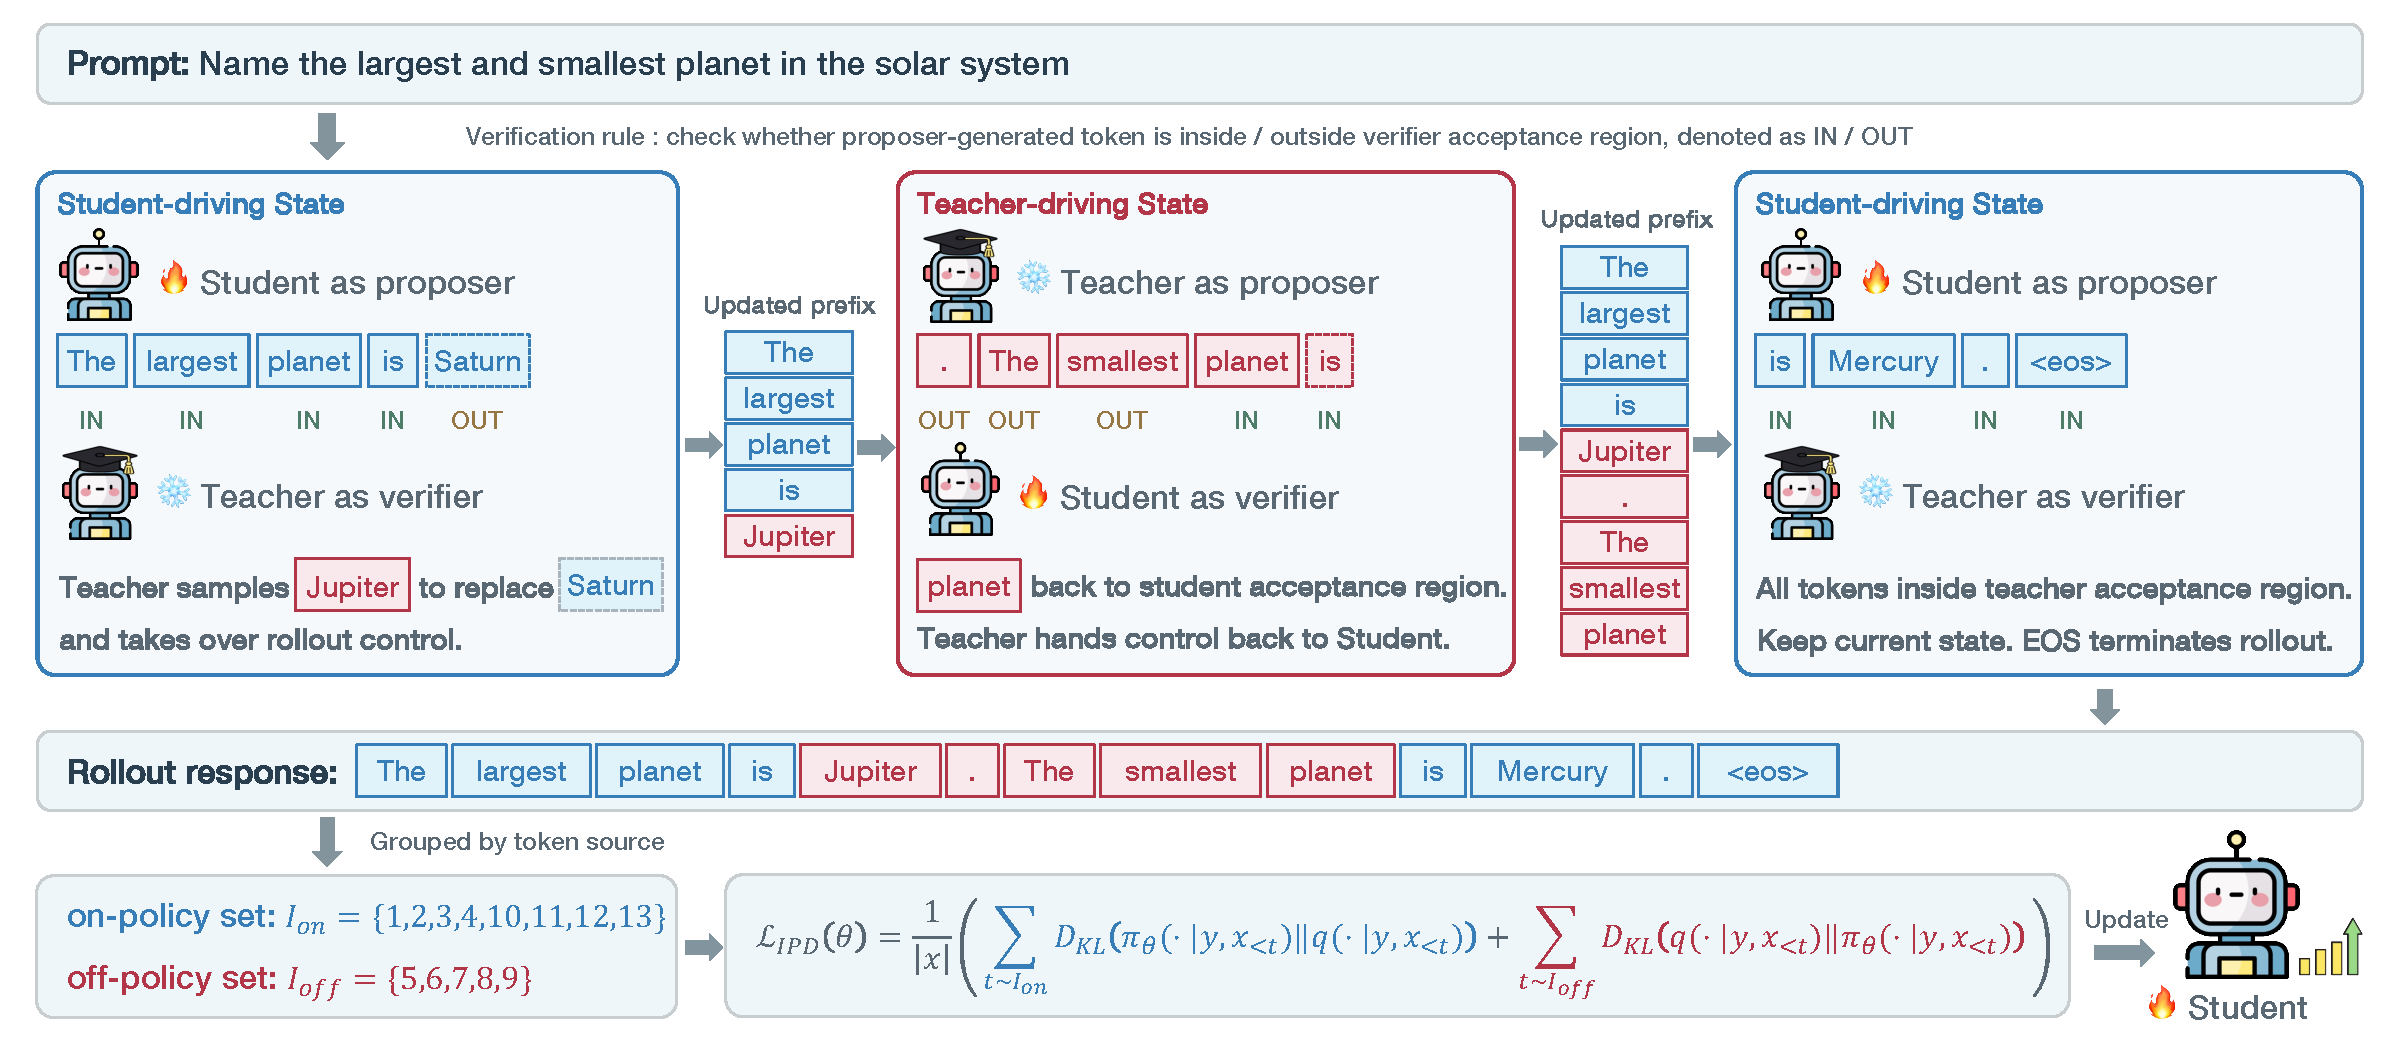
\includegraphics[width=0.99\textwidth]{figures/ipd_demo.pdf}
  \caption{The rollout and training demonstration of IPD. The student and teacher collaboratively generate the rollout under a bidirectional propose-and-verify state machine. Then tokens are grouped by their sources, and the IPD source-split loss is applied to update the student weights.}
  \label{fig:ipd_demo}
\end{figure}

However, student-generated trajectories can deviate far from the teacher when there is a large reasoning gap between them, and then the teacher is queried by states it would hardly visit and may provide unreliable learning signals \citep{ko2024distillm, skd}. We call this failure mode \emph{teacher unanchoring}. 
To overcome this challenge, we introduce \textbf{Interactive-Policy Distillation (IPD)}, which couples a bidirectional propose-and-verify state machine with different supervisions on tokens from different sources. As shown in Figure~\ref{fig:ipd_demo}, IPD allows the teacher to dynamically correct a drifting rollout and returns control once the corrected continuation falls within the student's acceptance region where student can actually resume. 
As the resulting trajectory interleaves the student's own decisions with teacher-provided corrective demonstrations, IPD assigns different supervisions by token sources, \emph{i.e.}, reverse KL at student-generated positions and forward KL at teacher-generated positions. Our contributions are summarized as follows:
\begin{itemize}[leftmargin=*]
    \setlength{\itemsep}{1pt}
    \setlength{\parsep}{0pt}
    \item We introduce IPD, a novel distillation algorithm with adaptive teacher intervention through a bidirectional propose-and-verify state machine, in which student and teacher dynamically exchange proposer and verifier roles. Its source-split objective applies reverse KL to student-generated positions and forward KL to teacher-generated positions, bridging on-policy and off-policy distillation paradigms.
    \item We design a fused inference engine, which co-hosts both models in one serving instance, maintains separate KV caches, and schedules requests according to their current proposer and verifier roles, to achieve more efficient dual-model scheduling during the rollout stage. 
    \item Empirically, across four teacher-student pairs on mathematical reasoning, IPD achieves the highest benchmark-averaged mean@8 and best@8 accuracy and leads on most individual benchmark metrics. Besides, IPD shows higher data efficiency. When distilling Qwen3-30B-A3B to Qwen3-1.7B-Base, IPD surpasses the mean@8 of OPD trained for a full epoch (279 steps) after only 60 training steps. We also demonstrate the robustness of IPD across different training datasets.
\end{itemize}


\section{Related Works}
\label{sec:related_works}

\noindent\textbf{On-policy distillation for LLMs.} LLM distillation used to be dominated by off-policy distillation on teacher-generated traces \citep{hinton2015distilling, kim2016sequence, guo2025deepseek}. The main weakness of off-policy distillation is that the student trains on teacher-authored prefixes but deploys on its own, and is vulnerable to exposure bias \citep{bengio2015scheduled, arora2022exposure}. 
GKD \citep{gkd} applies purely on-policy student sequences for training, and MiniLLM \citep{gu2024minillm} studies sequence-level reverse KL on those sequences. DistiLLM \citep{ko2024distillm} introduces skew divergences with an adaptive off-policy scheduler, and DistiLLM-2 \citep{ko2025distillm} contrasts teacher and student responses with skew forward and reverse KL.
% GKD \citep{gkd} brought student-generated sequences into distillation, while MiniLLM \citep{gu2024minillm} studied sequence-level reverse KL on those sequences. DistiLLM \citep{ko2024distillm, ko2025distillm} introduced skew divergences and adaptive scheduling.
%  and TAID \citep{shing2025taid} interpolates the target distribution to ease the capacity gap. 
Recently, OPD has already been incorporated as a core stage into reasoning-model post-training pipelines \citep{yang2025qwen3, lu2025onpolicydistillation, xiao2026mimo}.

\noindent\textbf{Challenges in on-policy distillation.}
Recent analyses characterize unreliable teacher feedback on student rollouts \citep{fu2026revisiting, armandpour2026unmasking, li2026rethinking}. EOPD \citep{jin2026entropyaware} adjusts the loss while retaining student-generated rollouts. TrOPD \citep{xing2026trust} uses a teacher-generated prefix followed by a student continuation and applies region-specific losses, but without dynamic teacher intervention during the continuation. SKD \citep{skd} adapts speculative propose-and-verify \citep{leviathan2023fast, chen2023accelerating} to rollout and implements dynamic teacher corrections. The student and teacher remain fixed roles as proposer and verifier. When a student token is rejected, the teacher resamples that position, and the student resumes generation from the corrected prefix.
Interactive imitation learning studies intervention and return of control through human judgment in HG-DAgger \citep{kelly2019hg} or uncertainty-based gating in EnsembleDAgger \citep{menda2019ensembledagger}. 
In contrast, IPD build a state machine model that dynamically swaps proposer and verifier roles through teacher takeover on rejected student tokens and handback on accepted teacher tokens, and then trains the resulting mixed-source trajectory with a source-split objective.

\section{Methodology}
\label{sec:method}

\subsection{Preliminaries}

Let $y\sim\mathcal{D}$ be a prompt from a dataset $\mathcal{D}$, $x=(x_1,\ldots,x_T)$ a response trajectory, and $c_t=(y,x_{<t})$ the prefix context at step $t$. The student and teacher next-token distributions are denoted as $\pi_\theta(\cdot\mid c_t)$ and $q(\cdot\mid c_t)$, and their complete-response probabilities factorize as $\pi_\theta(x\mid y)=\prod_{t=1}^{|x|}\pi_\theta(x_t\mid c_t)$ and $q(x\mid y)=\prod_{t=1}^{|x|}q(x_t\mid c_t)$.

% Throughout, \emph{sequence-level KL} denotes KL between complete-response distributions, whereas \emph{token-level KL} denotes conditional KL between next-token distributions at a fixed prefix. We call an aggregation of token-level terms along a sampled response a \emph{rollout-level loss}, not a third type of KL divergence.

\noindent\textbf{Off-Policy Distillation.}
Traditional knowledge distillation trains on prefixes sampled from a distribution $\mu$, which is typically a dataset of fixed reference responses or trajectories sampled from a teacher model \citep{hinton2015distilling, kim2016sequence}.  
Its standard objective is minimizing the forward KL, 
\begin{equation}
    \mathcal{L}_{\mathrm{off}}(\theta)
    = \mathbb{E}_{\substack{y\sim\mathcal{D}, x\sim \mu(\cdot\mid y)}}
    \left[
    \frac{1}{|x|}\sum_{t=1}^{|x|}
    D_{\mathrm{KL}}\!\left(
        q(\cdot\mid c_t)\,\Vert\,\pi_\theta(\cdot\mid c_t)
    \right)
    \right].
    \label{eq:off_policy_kd}
\end{equation}
The fixed prefixes make optimization stable and permit dense supervision over the vocabulary, but they also induce a state-distribution mismatch: at inference time, the student must condition on its own previous tokens, including mistakes that are absent from teacher-generated trajectories.

\noindent\textbf{On-Policy Distillation.}
Compared with off-policy distillation, on-policy distillation (OPD) evaluates teacher feedback on responses sampled from the student itself \citep{gkd, gu2024minillm}. Under the notations above, its theoretical objective is the sequence-level reverse KL
\begin{equation}
    \mathcal{L}^{\mathrm{seq}}_{\mathrm{on}}(\theta)
    = \mathbb{E}_{y\sim\mathcal{D}}
    \left[
      D_{\mathrm{KL}}\!\left(
        \pi_\theta(\cdot\mid y)\,\Vert\,q(\cdot\mid y)
      \right)
    \right] 
    = \mathbb{E}_{\substack{y\sim\mathcal{D}, x\sim\pi_\theta(\cdot\mid y)}}
    \left[
      \sum_{t=1}^{|x|} D_{\mathrm{KL}}\!\left(
        \pi_\theta(\cdot\mid c_t)\,\Vert\,q(\cdot\mid c_t)
      \right)
    \right],
    \label{eq:on_policy_kd}
\end{equation}
The outer expectation samples prefixes from the student-induced state distribution, while each summand is a token-level conditional reverse KL at one such prefix. 
% The sum is not divided by $|x|$ because length normalization would define a different rollout-level objective rather than the sequence-level KL on the left-hand side.
At a fixed prefix $c_t$, the exact token-level conditional reverse KL is computed over the entire vocabulary $\mathcal{V}$ as
\begin{equation}
    \ell^{\mathrm{full}}_t(\theta) 
    = D_{\mathrm{KL}}\!\left(
      \pi_\theta(\cdot\mid c_t)\,\Vert\,q(\cdot\mid c_t)
      \right) 
    = \sum_{v\in\mathcal{V}}\pi_\theta(v\mid c_t) \log\frac{\pi_\theta(v\mid c_t)}{q(v\mid c_t)}.
    \label{eq:full_vocab_opd}
\end{equation}
Optimizing Eq.~(\ref{eq:full_vocab_opd}) requires forward and backward passes over all $|\mathcal{V}|$ indices at every position, which is computationally expensive \citep{li2026rethinking, oh2026klforkl}.

\noindent\textbf{Sampled-Token and Top-$K$ OPD.}
As a less expensive alternative to the full-vocabulary KL in Eq.~(\ref{eq:full_vocab_opd}), sampled-token OPD evaluates only the student-sampled token $x_t\sim\pi_\theta(\cdot\mid c_t)$. The resulting single-sample Monte Carlo estimate of the token-level KL value at the fixed prefix $c_t$ is
\begin{equation}
    \widehat{\ell}^{\mathrm{sample}}_t
    =\log \pi_\theta(x_t\mid c_t)-\log q(x_t\mid c_t).
    \label{eq:sampled_token_opd}
\end{equation}

Although Eq.~(\ref{eq:sampled_token_opd}) is an unbiased estimate for the full-vocabulary KL, the variance introduced by sampling a single token can make updates noisy and unstable \citep{oh2026klforkl}. 
Top-$K$ OPD reaches a sweet spot between full-vocabulary and sampled-token OPD. It retains multi-token supervision on a small high-probability support while avoiding a full-vocabulary computation \citep{li2026rethinking, fu2026revisiting}. 
Let
\begin{equation}
    S_t^{\pi}=\operatorname{Top}_K\!\left(
      \pi_\theta(\cdot\mid c_t)\right),
    \qquad
    S_t^{q}=\operatorname{Top}_K\!\left(q(\cdot\mid c_t)\right),
    \label{eq:topk_sets}
\end{equation}
denote the student and teacher top-$K$ supports, respectively, where $\operatorname{Top}_K$ returns the $K$ highest-probability indices, and denote $S_t\subseteq\mathcal{V}$ as the support for distillation, which can usually be $S_t^{\pi}$, $S_t^{q}$, $S_t^{\pi} \cup S_t^{q}$, or $S_t^{\pi} \cap S_t^{q}$. As the two models generally assign different total probability mass to $S_t$, each distribution should be normalized by 
\begin{equation}
    \bar{\pi}^{S_t}_\theta(v\mid c_t) = \frac{\pi_\theta(v\mid c_t)\mathds{1}[v\in S_t]}{\sum_{u\in S_t}\pi_\theta(u\mid c_t)}, \quad
    \bar{q}^{S_t}(v\mid c_t) = \frac{q(v\mid c_t)\mathds{1}[v\in S_t]}{\sum_{u\in S_t}q(u\mid c_t)}.
    \label{eq:topk_normalization}
\end{equation}
Then, the token-level top-$K$ KL and its rollout-level aggregated loss are given by
\begin{gather}
    \ell^{\mathrm{top}\text{-}K}_t(\theta;S_t)
    =D_{\mathrm{KL}}\!\left(
      \bar{\pi}^{S_t}_\theta(\cdot\mid c_t)
      \,\Vert\,\bar{q}^{S_t}(\cdot\mid c_t)\right) = \sum_{v\in S_t}\bar{\pi}^{S_t}_\theta(v\mid c_t) \log\frac{\bar{\pi}^{S_t}_\theta(v\mid c_t)} {\bar{q}^{S_t}(v\mid c_t)}, \label{eq:topk_opd_on_sequence}\\
    \mathcal{L}^{\mathrm{top}\text{-}K}_{\mathrm{on}}(\theta)
    =\mathbb{E}_{\substack{y\sim\mathcal{D}, x\sim\pi_\theta(\cdot\mid y)}}
      \left[\sum_{t=1}^{|x|} \ell^{\mathrm{top}\text{-}K}_t(\theta;S_t)\right].
    \label{eq:topk_opd}
\end{gather}
Although top-$K$ OPD is a biased approximation to full-vocabulary OPD as it discards probability mass outside $S_t$, it replaces the high-variance single-token estimate of sampled-token OPD with deterministic multi-token supervision over the selected high-probability support for each fixed prefix $c_t$, and therefore provides a practical middle ground with denser and more stable supervision than sampled-token OPD \citep{fu2026revisiting}, while at the same time reducing the per-token computation and backward-pass cost of full-vocabulary OPD \citep{li2026rethinking, oh2026klforkl}.

\subsection{Interactive-Policy Distillation}

Vanilla OPD samples trajectories from the student, and the teacher feedback is evaluated on states that may be far from where it would actually visit. We name it as \emph{teacher unanchoring}. Figure~\ref{fig:teacher_unanchoring_example} illustrates the average entropy and reverse KL over position intervals on the student (Qwen3-1.7B-Base) responses for 512 randomly selected DAPO-MATH-17K \citep{yu2025dapo} prompts, split by the final answer correctness. The teacher (Qwen3-30B-A3B non-thinking) queried by incorrect trajectories yields high uncertainty, even as the reverse KL decays along the position. We propose Interactive-Policy Distillation (IPD), which formulates generation as a state machine in which the student and teacher alternate as proposer and verifier. to address this challenge by dynamic adaptive teacher intervention during rollout. 

\begin{figure}[!t]
  \centering
  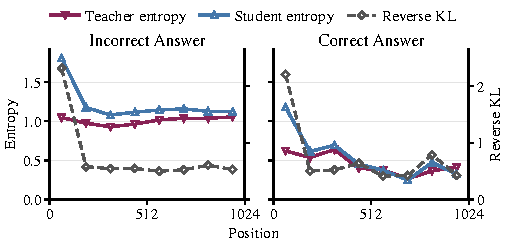
\includegraphics[width=0.6\textwidth]{figures/teacher_unanchoring_example.pdf}
  \caption{Average entropy and reverse KL over position intervals on the student responses split by the final answer correctness.}
  % Average entropy and reverse KL over position intervals on the student (Qwen3-1.7B-Base) responses for 512 randomly selected DAPO-MATH-17K prompts, split by the final answer correctness. The teacher (Qwen3-30B-A3B non-thinking) is less certain on incorrect prefixes, while the reverse KL still decays along position.
  \label{fig:teacher_unanchoring_example}
\end{figure}

\subsubsection{Adaptive Teacher Intervention with Bidirectional Propose-and-Verify}

Let $m_t\in\{\mathsf{S},\mathsf{T}\}$ denote the driver model state before generating token at position $t$, where $\mathsf{S}$ and $\mathsf{T}$ indicate student driving and teacher driving, respectively, and we initialize every rollout with $m_1=\mathsf{S}$. Let $z_t\in\{\mathsf{S},\mathsf{T}\}$ record the source of the token actually emitted at position $t$. We use top-$K$ coverage as the takeover and handback rules, with $S_t^\pi$ and $S_t^q$ defined in Eq.~(\ref{eq:topk_sets}).
%  and $K=16$ by default.

\noindent\textbf{Student driving.} When $m_t=\mathsf{S}$, the student proposes $\widetilde{x}_t^\pi\sim\pi_\theta(\cdot\mid c_t)$ and the teacher verifies whether the student-generated token is covered by the teacher's top-$K$ support, \emph{i.e.,} $\widetilde{x}_t^\pi \in S_t^q$. If covered, which indicates that the student's proposal within the teacher's acceptance region, IPD accepts the student proposal, assigns $z_t=\mathsf{S}$, and remains in student driving state. Otherwise, the proposal is discarded, and the teacher samples a replacement $\widetilde{x}_t^q\sim q(\cdot\mid c_t)$. IPD emits this teacher-sampled token with $z_t=\mathsf{T}$, and the rollout control switches to the teacher from position $t+1$.

\noindent\textbf{Teacher driving.} When $m_t=\mathsf{T}$, the teacher proposes $\widetilde{x}_t^q\sim q(\cdot\mid c_t)$ and the student verifies whether the teacher-sampled token satisfies $\widetilde{x}_t^q\in S_t^\pi$. If it is not covered by the student's top-$K$ support, the teacher retains control. Otherwise, as the teacher's proposal is back to the student's acceptance region, which indicates that the student is possible to generate is on its own, it is kept and serves as the handback trigger and the rollout control is returned to student rom position $t+1$.

The complete per-token transition can be written as
\begin{equation}
    (x_t,z_t,m_{t+1})=
    \begin{cases}
        (\widetilde{x}_t^\pi,\mathsf{S},\mathsf{S}), & m_t=\mathsf{S},\ \widetilde{x}_t^\pi\in S_t^q,\\
        (\widetilde{x}_t^q,\mathsf{T},\mathsf{T}), & m_t=\mathsf{S},\ \widetilde{x}_t^\pi\notin S_t^q,\\
        (\widetilde{x}_t^q,\mathsf{T},\mathsf{S}), & m_t=\mathsf{T},\ \widetilde{x}_t^q\in S_t^\pi,\\
        (\widetilde{x}_t^q,\mathsf{T},\mathsf{T}), & m_t=\mathsf{T},\ \widetilde{x}_t^q\notin S_t^\pi.
    \end{cases}
    \label{eq:ipd_state_transition}
\end{equation}
The state machine iterates until an EOS token is emitted or the maximum rollout length is reached. Eq.~(\ref{eq:ipd_state_transition}) is written token by token for clarity. Following \citet{leviathan2023fast} and \citet{skd}, for a faster rollout, the implementation usually consecutively proposes a chunk of $\gamma$ tokens and verify them in parallel, instead of token-by-token verification immediately after decoded. 

Note that in this paper we use the top-$K$ coverage as the takeover and handback rules. As a unified framework, IPD is also compatible with other rules, and the takeover and handback rules can also be asymmetric. For example, we can instead use a threshold on the entropy of the student or the teacher distributions to determine whether to take over or hand back control. SKD \citep{skd} can be included as a special case of IPD with a top-$K$ coverage takeover rule and a fixed-one-token handback rule, and in our experiments, SKD is also implemented under our customized fused engine for more efficient rollout.

\subsubsection{Source-Split KL Objective}

The state machine model formulated by Eq.~(\ref{eq:ipd_state_transition}) produces a response trajectory $x$ together consisting of student-generated and teacher-generated tokens with recorded source labels $z=(z_1,\ldots,z_{T})$. Denote $I_{on}(z)=\{t:z_t=\mathsf{S}\}$ and $I_{off}(z)=\{t:z_t=\mathsf{T}\}$ as the on-policy (student-generated) and off-policy (teacher-generated) position sets, respectively. Since the trajectory $x$ is a mixure of student and teacher tokens, it is natural provide the two groups of positions with different supervisions. We therefore design a source-split KL objective that applies different KL divergences to student-generated and teacher-generated positions.

Specifically, the token-level KL divergences applied to student-generated and teacher-generated positions are respectively denoted as 
\begin{align}
    \ell_t^{\mathrm{on}}(\theta)
    =D_{\mathrm{KL}}\!\left(\bar{\pi}^{S_t}_\theta(\cdot\mid c_t)\,\Vert\,\bar{q}^{S_t}(\cdot\mid c_t)\right), \quad
    \ell_t^{\mathrm{off}}(\theta)
    =D_{\mathrm{KL}}\!\left(\bar{q}^{S_t}(\cdot\mid c_t)\,\Vert\,\bar{\pi}^{S_t}_\theta(\cdot\mid c_t)\right). \label{eq:ipd_off_loss}
\end{align}
Student-generated positions therefore receive the token-level reverse KL used by on-policy distillation, while teacher-generated tokens receive the token-level forward KL used by off-policy distillation. Both losses are evaluated at the realized mixed-source prefix $c_t$, regardless of which model generated earlier tokens.
Let $\rho_\theta^{\mathrm{IPD}}(x,z\mid y)$ denote the joint distribution over emitted responses and source labels induced by the state machine in Eq.~(\ref{eq:ipd_state_transition}). The final length-normalized objective is minimizing the following source-split KL
\begin{equation}
    \mathcal{L}_{\mathrm{IPD}}(\theta)=\mathbb{E}_{\substack{y\sim\mathcal{D},\,(x,z)\sim\rho_\theta^{\mathrm{IPD}}(\cdot,\cdot\mid y)}}\!\left[\frac{1}{|x|}\left(\sum_{t\in I_{on}(z)}\ell_t^{\mathrm{on}}(\theta)+\sum_{t\in I_{off}(z)}\ell_t^{\mathrm{off}}(\theta)\right)\right].
    \label{eq:ipd_objective}
\end{equation}

With the bidirectional propose-and-verify mechanism and the source-split KL, IPD naturally becomes a unified bridge between on-policy and off-policy distillations. Specifically, never transferring control to the teacher yields length-normalized on-policy distillation with reverse KL supervision on pure student-generated trajectories, while always rejecting the first student proposal and never handing control back yields off-policy distillation with forward KL supervision on pure teacher-generated trajectories.

\subsubsection{Fused Inference Engine for Efficient Dual-Model Scheduling}

\begin{wrapfigure}{r}{0.45\textwidth}
  \centering
  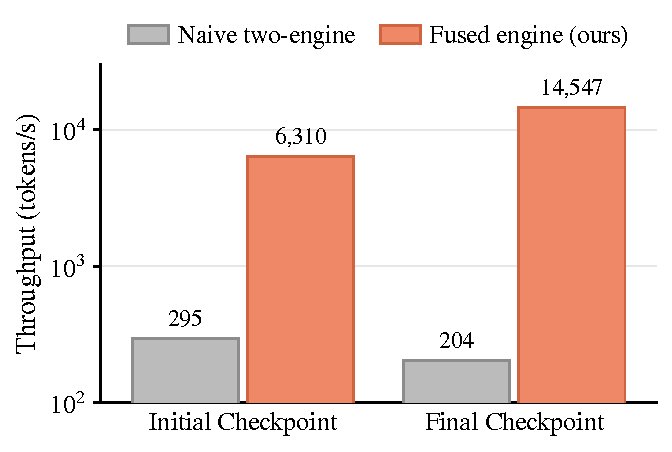
\includegraphics[width=\linewidth]{figures/throughput_fused_vs_naive.pdf}
  \setlength{\abovecaptionskip}{5pt}
  \vspace{-10pt}
  \caption{IPD rollout throughput of fused engine and naive two-engine implementation.}
  % \vspace{-10pt}
  \label{fig:fused_vs_naive_throughput}
\end{wrapfigure}

To integrate IPD with verl \citep{sheng2025hybridflow}, built on vLLM \citep{kwon2023efficient}, we design a fused inference engine for more efficient dual-model scheduling. 
A naive implementation that hosts two models on separate vLLM serving instances will have to re-encode the whole prefix for every verification round, as an off-the-shelf vLLM engine bypasses its prefix cache for requests that return prompt log-probabilities and cannot append externally generated tokens to the KV cache of a live request. Besides, there are also communication overheads between two engines. 
% The fused engine removes those cost by keeping both models' KV caches for the same sequence in a single engine and extending them incrementally with each other's tokens. 
As shown in Figure~\ref{fig:fused_vs_naive_throughput}, with Qwen3-4B-Base (non-thinking) as the teacher and Qwen3-1.7B-Base as the student, executing the IPD rollout with bidirectional propose-and-verify on the same 512 randomly selected DAPO-MATH-17K prompts under identical settings and memory budget, fused engine is 21.4$\times$ faster than the naive implementation on the initial checkpoint and 71.4$\times$ faster on the final one. 

Specifically, as illustrated in Figure~\ref{fig:fused_engine_step}, our fused engine co-hosts the student and teacher in one serving instance, and each active request maintains a verified prefix, a chunk of unverified draft tokens, the identity of its current driver model, and separate student and teacher KV-cache states. 
For each request, the two models serve as symmetrical roles. Each model maintains its own cache and may act as either the proposer or the verifier, with the verifier always being the counterpart of the current driver model.
One fused engine step consists of a verification, a verdict, and a proposal stage. In the verification stage, requests are grouped by their verifier, and each verifier evaluates all unverified draft tokens of its sub-batch in parallel through a single prefill pass. Only the newly appended tokens require computation as long as the cache of the verified prefix remains resident. If vLLM preempts a request under resource contention and evicts its cached blocks, the affected model, whether verifier or proposer, will instead recompute the KV states of the whole prefix. 
In the verdict stage, the engine determines the acceptance or rejection of each draft, detects takeover and handback transitions, updates the driver model, and aligns both KV caches with the resulting verified prefix. If no transition occurs, all drafted tokens are kept and both caches are preserved. If a student token triggers takeover, the token is rejected and will be regenerated by the teacher, so both caches are rolled back to the preceding token. If a teacher token triggers handback, the token is retained, so both caches are rolled back only to it and the subsequent draft tokens are discarded. Either way, the two caches end at the same accepted-prefix boundary. 
In the proposal stage, requests are regrouped by their updated driver model, and each proposer autoregressively decodes a new chunk of $\gamma$ draft tokens for its sub-batch while extending only its own KV cache, leaving the counterpart model to catch up through the prefill of the next verification stage. Consequently, apart from draft tokens discarded by a transition and cache blocks evicted by preemption, every token is decoded once by its proposer and prefilled once by its verifier. The engine repeats these stages until every request has emitted an accepted EOS token or reached the maximum generation length. A student-generated EOS token terminates the request only if it passes the teacher's takeover test and otherwise triggers a teacher takeover at that position, whereas a teacher-generated EOS token is accepted directly.

\begin{figure}[!h]
  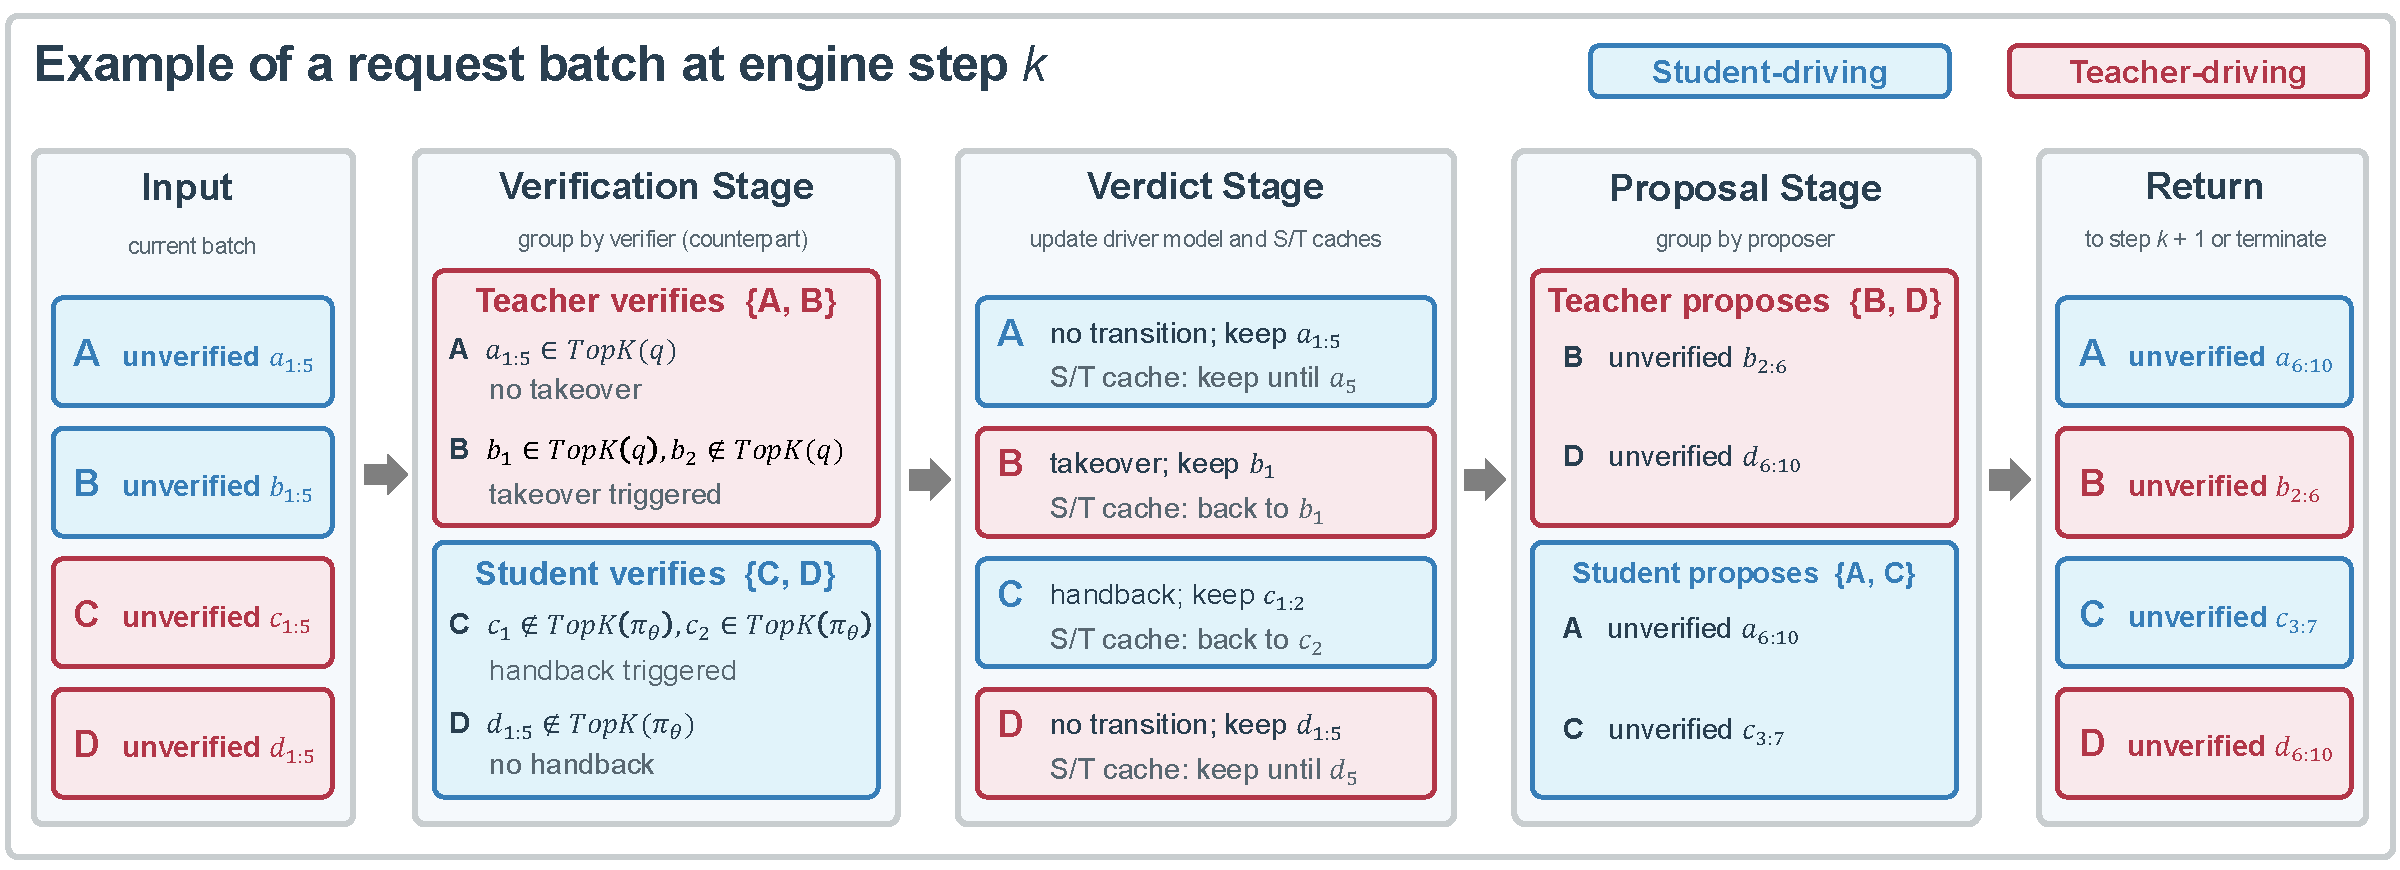
\includegraphics[width=0.99\textwidth]{figures/fused_engine.pdf}
  \caption{Example of one IPD fused engine step for a request batch. The engine distributes requests to their respective verifier models for verification, collects verification results, updates their driver models, manages their KV cache on each model, re-distributes requests to their respective proposer models for new unverified draft tokens, and return the updated requests for next step or termination.}
  \label{fig:fused_engine_step}
\end{figure}

\section{Experiments}
\label{sec:exp}

\subsection{Experimental Settings}
We train four Qwen3 \citep{yang2025qwen3} teacher-student pairs on DAPO-Math-17K~\citep{yu2025dapo} for one epoch, with thinking mode disabled for all teachers. We set $K=16$: all methods apply distillation over the union support $S_t=S_t^\pi\cup S_t^q$, and IPD and SKD use top-$K$ coverage for takeover, with IPD also using it for handback. We use the codebase from \citet{li2026rethinking} for OPD, and additionally build our fused inference engine and implement SKD and IPD training pipelines on top of that. Both IPD and SKD use a proposal chunk length of $\gamma=5$. We evaluate the final checkpoints on six mathematical reasoning benchmarks and report mean@8 and best@8 accuracy. Appendix~\ref{sec:full_exp_details} provides more detailed model, training, hardware, and evaluation configurations.

\begin{table}[!h]
\setlength{\abovecaptionskip}{0pt}
\setlength{\aboverulesep}{0pt}
\setlength{\belowrulesep}{0pt}
\setlength{\extrarowheight}{2pt}
\centering
\small
\caption{Comparison of different distillation methods across various student and teacher model combinations. We report mean@8 and best@8 accuracy (\%) on different math reasoning benchmarks, as well as the benchmark-wise average.}
\label{tab:main_results}
\resizebox{\textwidth}{!}{%
\begin{tabular}{ll cc cc cc cc cc cc cc}
\toprule
\multicolumn{1}{c}{\multirow{2}{*}{\makecell{Teacher/\\Student}}} & \multicolumn{1}{c}{\multirow{2}{*}{Method}} & \multicolumn{2}{c}{MATH-500} & \multicolumn{2}{c}{Minerva} & \multicolumn{2}{c}{Olympiad} & \multicolumn{2}{c}{AMC23} & \multicolumn{2}{c}{AIME24} & \multicolumn{2}{c}{AIME25} & \multicolumn{2}{c}{\textbf{Avg.}} \\
\cmidrule(lr){3-4} \cmidrule(lr){5-6} \cmidrule(lr){7-8} \cmidrule(lr){9-10} \cmidrule(lr){11-12} \cmidrule(lr){13-14} \cmidrule(lr){15-16}
& & mean@8 & best@8 & mean@8 & best@8 & mean@8 & best@8 & mean@8 & best@8 & mean@8 & best@8 & mean@8 & best@8 & mean@8 & best@8 \\
\midrule
\multirow{3}{*}{\makecell[l]{Qwen3-4B/\\Qwen3-1.7B-Base}} & OPD & 66.68 & 84.06 & 26.42 & 44.04 & 31.00 & 48.45 & 35.69 & \textbf{57.29} & 7.92 & \textbf{21.77} & 2.92 & 8.70 & 28.44 & 44.05 \\
 & SKD & 66.70 & 84.50 & 27.94 & 43.69 & 29.75 & 49.52 & 35.09 & 52.90 & 8.75 & 17.41 & 4.58 & 10.73 & 28.80 & 43.13 \\
& \ipdcell{\textbf{IPD (ours)}} & \ipdcell{\textbf{69.28}} & \ipdcell{\textbf{84.59}} & \ipdcell{\textbf{29.60}} & \ipdcell{\textbf{46.26}} & \ipdcell{\textbf{31.80}} & \ipdcell{\textbf{49.63}} & \ipdcell{\textbf{36.14}} & \ipdcell{57.25} & \ipdcell{\textbf{9.17}} & \ipdcell{21.69} & \ipdcell{\textbf{6.67}} & \ipdcell{\textbf{15.06}} & \ipdcell{\textbf{30.44}} & \ipdcell{\textbf{45.75}} \\
\midrule
\multirow{3}{*}{\makecell[l]{Qwen3-30B-A3B/\\Qwen3-1.7B-Base}} & OPD & 63.35 & 83.54 & 23.25 & 41.43 & 28.14 & 46.88 & 32.68 & 54.39 & 10.42 & 18.84 & \textbf{5.83} & 13.12 & 27.28 & 43.03 \\
 & SKD & 67.38 & 84.34 & 26.70 & 44.69 & 30.39 & 49.73 & 33.89 & 54.67 & 8.75 & 22.36 & \textbf{5.83} & \textbf{14.92} & 28.82 & 45.12 \\
& \ipdcell{\textbf{IPD (ours)}} & \ipdcell{\textbf{69.35}} & \ipdcell{\textbf{84.61}} & \ipdcell{\textbf{29.60}} & \ipdcell{\textbf{46.44}} & \ipdcell{\textbf{32.56}} & \ipdcell{\textbf{51.29}} & \ipdcell{\textbf{34.79}} & \ipdcell{\textbf{59.60}} & \ipdcell{\textbf{11.67}} & \ipdcell{\textbf{22.79}} & \ipdcell{5.42} & \ipdcell{13.10} & \ipdcell{\textbf{30.56}} & \ipdcell{\textbf{46.31}} \\
\midrule
\multirow{3}{*}{\makecell[l]{Qwen3-8B/\\Qwen3-4B-Base}} & OPD & 79.63 & 90.83 & 36.53 & 52.22 & 44.80 & 60.49 & 44.28 & 66.31 & 15.83 & 25.40 & 13.75 & 29.09 & 39.14 & 54.06 \\
 & SKD & 80.43 & 91.49 & \textbf{37.91} & 51.15 & 44.71 & 61.32 & \textbf{51.51} & \textbf{72.01} & 15.42 & 24.76 & 15.00 & \textbf{29.68} & 40.83 & 55.07 \\
& \ipdcell{\textbf{IPD (ours)}} & \ipdcell{\textbf{81.45}} & \ipdcell{\textbf{92.21}} & \ipdcell{37.87} & \ipdcell{\textbf{52.66}} & \ipdcell{\textbf{46.43}} & \ipdcell{\textbf{62.19}} & \ipdcell{48.34} & \ipdcell{67.83} & \ipdcell{\textbf{17.08}} & \ipdcell{\textbf{28.86}} & \ipdcell{\textbf{17.08}} & \ipdcell{28.66} & \ipdcell{\textbf{41.38}} & \ipdcell{\textbf{55.40}} \\
\midrule
\multirow{3}{*}{\makecell[l]{Qwen3-30B-A3B/\\Qwen3-4B-Base}} & OPD & 81.38 & 90.00 & 39.11 & 53.41 & 46.66 & 61.18 & 48.80 & 67.88 & 15.42 & 24.78 & 12.92 & 26.36 & 40.71 & 53.93 \\
 & SKD & 81.03 & 91.96 & 40.40 & 55.39 & 47.42 & \textbf{63.95} & \textbf{49.85} & \textbf{72.82} & 16.25 & 24.85 & \textbf{16.67} & \textbf{27.60} & 41.93 & 56.09 \\
& \ipdcell{\textbf{IPD (ours)}} & \ipdcell{\textbf{82.28}} & \ipdcell{\textbf{92.40}} & \ipdcell{\textbf{41.18}} & \ipdcell{\textbf{55.52}} & \ipdcell{\textbf{47.66}} & \ipdcell{63.45} & \ipdcell{49.55} & \ipdcell{70.64} & \ipdcell{\textbf{19.58}} & \ipdcell{\textbf{28.39}} & \ipdcell{13.75} & \ipdcell{26.22} & \ipdcell{\textbf{42.33}} & \ipdcell{\textbf{56.10}} \\
\bottomrule
\end{tabular}}
\end{table}

\subsection{Main Results}

We compare IPD with OPD \citep{lu2025onpolicydistillation,li2026rethinking} and SKD \citep{skd} on multiple student and teacher model combinations across different sizes. Thinking mode is disabled for all non-base teachers. In Table~\ref{tab:main_results}, our algorithm demonstrates consistent improvements over the baselines across all benchmarks and model combinations. Specifically, when distilling Qwen3-4B to Qwen3-1.7B-Base, IPD achieves an average mean@8 accuracy of $30.44$ across all benchmarks, outperforming OPD and SKD by $+2.00$ and $+1.64$, respectively. Besides, IPD also allows the student to robustly learn from a larger teacher. According to the discussion in \citet{li2026rethinking}, a larger teacher cannot always distill a better student, and when the teacher-student reasoning gap is too large, the distillation performance can be suboptimal. In our experiments, when distilling Qwen3-30B-A3B to Qwen3-1.7B-Base, we also find this phenomenon that the distilled student achieves an average mean@8 accuracy of $27.28$, which is lower than the $28.44$ achieved by distilling a Qwen3-4B teacher. Meanwhile, with the bidirectional propose-and-verify mechanism, IPD can effectively bridge the reasoning gap between the teacher and student, achieving an average mean@8 accuracy of $30.56$, which is $3.28$ higher than OPD and $1.74$ higher than SKD. 

Besides, IPD is also a more data-efficient distillation algorithm. As shown in Figure~\ref{fig:main_training_curve}, IPD shows a much faster convergence than other baselines. Specifically, trained with only fewer than 1/4 training examples for 60 training steps, IPD can outperform OPD and matches SKD trained for a whole epoch with 279 training steps. Besides, IPD shows a stably increasing top-$K$ overlap ratio (defined by $\vert S^\pi_t \cap S^q_t \vert / K$), indicating a healthy training under large a teacher-student gap \citep{li2026rethinking}.

\begin{figure}[!h]
    \centering
    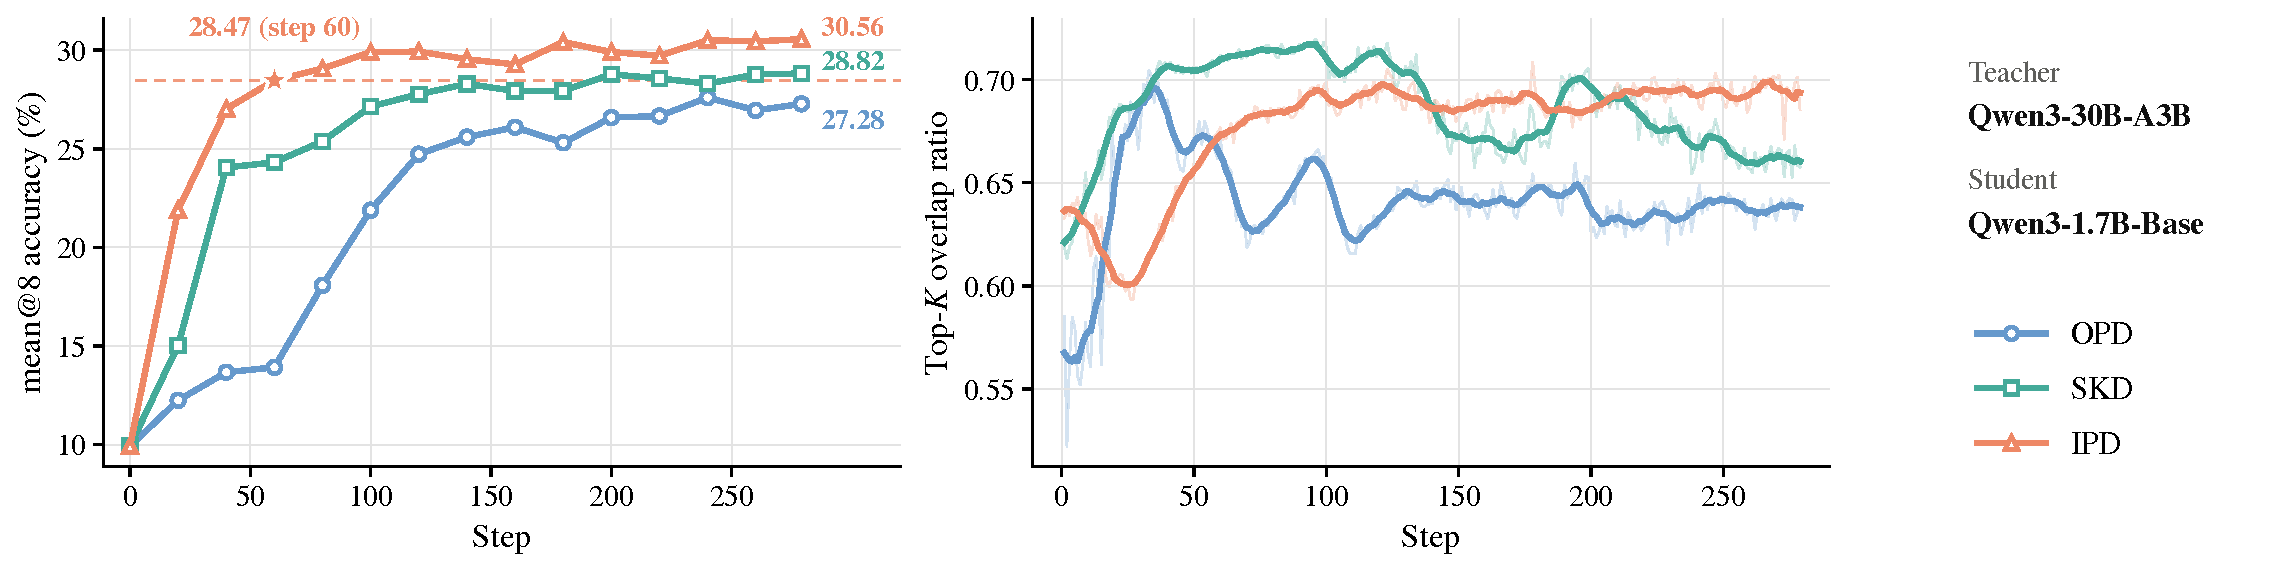
\includegraphics[width=0.99\linewidth]{figures/curves_1p7b_from_30b.pdf}
    \caption{The mean@8 accuracy over math reasoning benchmarks and top-$K$ overlap ratio during training on DAPO-MATH-17K. In addition to better final checkpoint performance, IPD also shows a much higher data efficiency than other baselines.}
    \label{fig:main_training_curve}
\end{figure}

\subsection{Ablation Study}

\noindent\textbf{KL direction.} To investigate the impact of different KL directions for on-policy and off-policy positions, and the resonability of our source-split KL design, we conduct an ablation study on the IPD KL objective. We compare the following configurations: 
(i) Forward KL for all positions (Pure Forward KL), (ii) Reverse KL for all positions (Pure Reverse KL), (iii) Forward KL for on-policy and Reverse KL for off-policy positions (Inverse-IPD-Split KL), and (iv) Reverse KL for on-policy and Forward KL for off-policy positions (IPD-Split KL, default).
As shown in Figure~\ref{fig:ablation_loss}, we observe that the IPD Default configuration, which uses Reverse KL for on-policy positions and Forward KL for off-policy positions, achieves the best mean@8 accuracy. Meanwhile, Pure Reverse KL turns out to be the runner-up, with the second-best mean@8 accuracy and a $0.12$ higher best@8 accuracy than the default source-split KL. The teacher intervention ratio, which is calculated by the proportion of teacher-generated tokens among all tokens, gradually decreases during training, indicating that the student is learning to generate more tokens that are covered by the teacher's top-$K$ support, and leaning more towards on-policy paradigm.

\begin{figure}[!h]
  \centering
  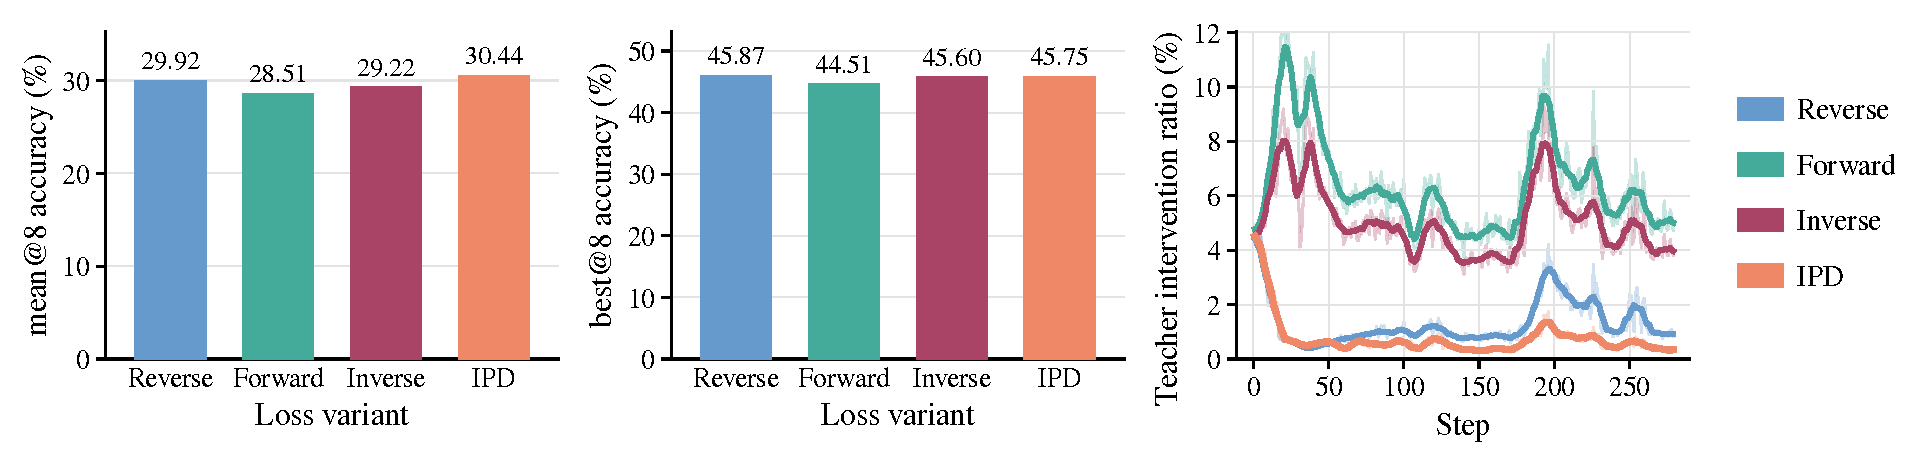
\includegraphics[width=0.99\linewidth]{figures/loss_ablation_triptych.pdf}
  \caption{The mean@8 and best@8 average accuracy over benchmarks and the teacher intervention ratio with different losses during IPD training.}
  \label{fig:ablation_loss}
\end{figure}


\noindent\textbf{Coverage width.}
In our main experiments, we set $K=16$ for the top-$K$ coverage takeover and handback rules in the IPD framework. Under a smaller $K$, there will be more teacher takeovers and less frequent teacher handbacks, which leans more towards off-policy training, results in a higher teacher invervention ratio during the rollout stage, and requires more computational resources. While under a larger $K$, the teacher will invervene less, leaning more towards an on-policy training. To study the effect of different coverage widths, we further conduct experiments with $K=4$, $K=8$, and $K=32$. 
As shown in Figure~\ref{fig:ablation_k_values}, IPD under $K=4$ achieves the best performance with $30.46$ mean@8 and $45.80$ best@8. The default $K=16$ appears to be a close runner-up with only $-0.02$ mean@8 and $-0.05$ best@8 gap, while getting much lower teacher intervention ratio, which provides a good balance between performance and computational efficiency.

\begin{figure}[!h]
  \centering
  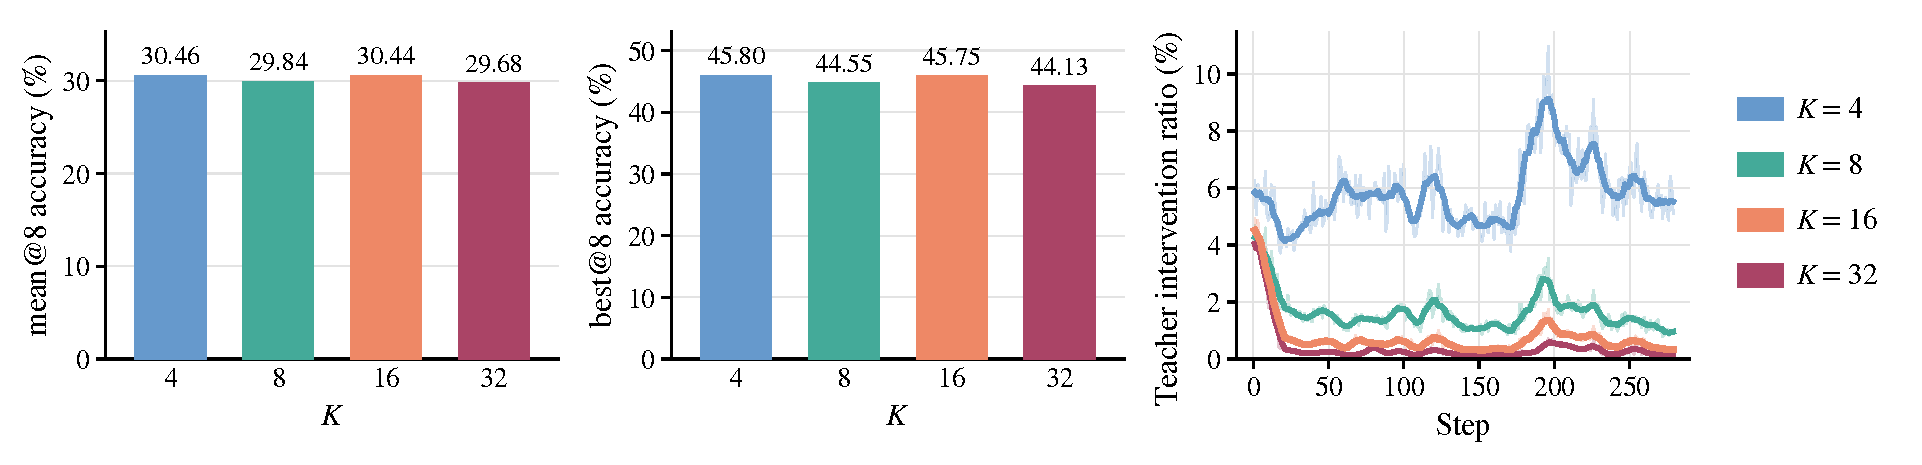
\includegraphics[width=0.99\linewidth]{figures/k_ablation_triptych.pdf}
  \caption{The mean@8 and best@8 average accuracy over benchmarks and the teacher intervention ratio with different coverage widths $K$ during IPD training. A smaller $K$ leads to more frequent teacher takeovers and less frequent teacher handbacks, resulting in a higher intervention ratio.}
  \vspace{-8pt}
  \label{fig:ablation_k_values}
\end{figure}

\begin{figure}[!h]
  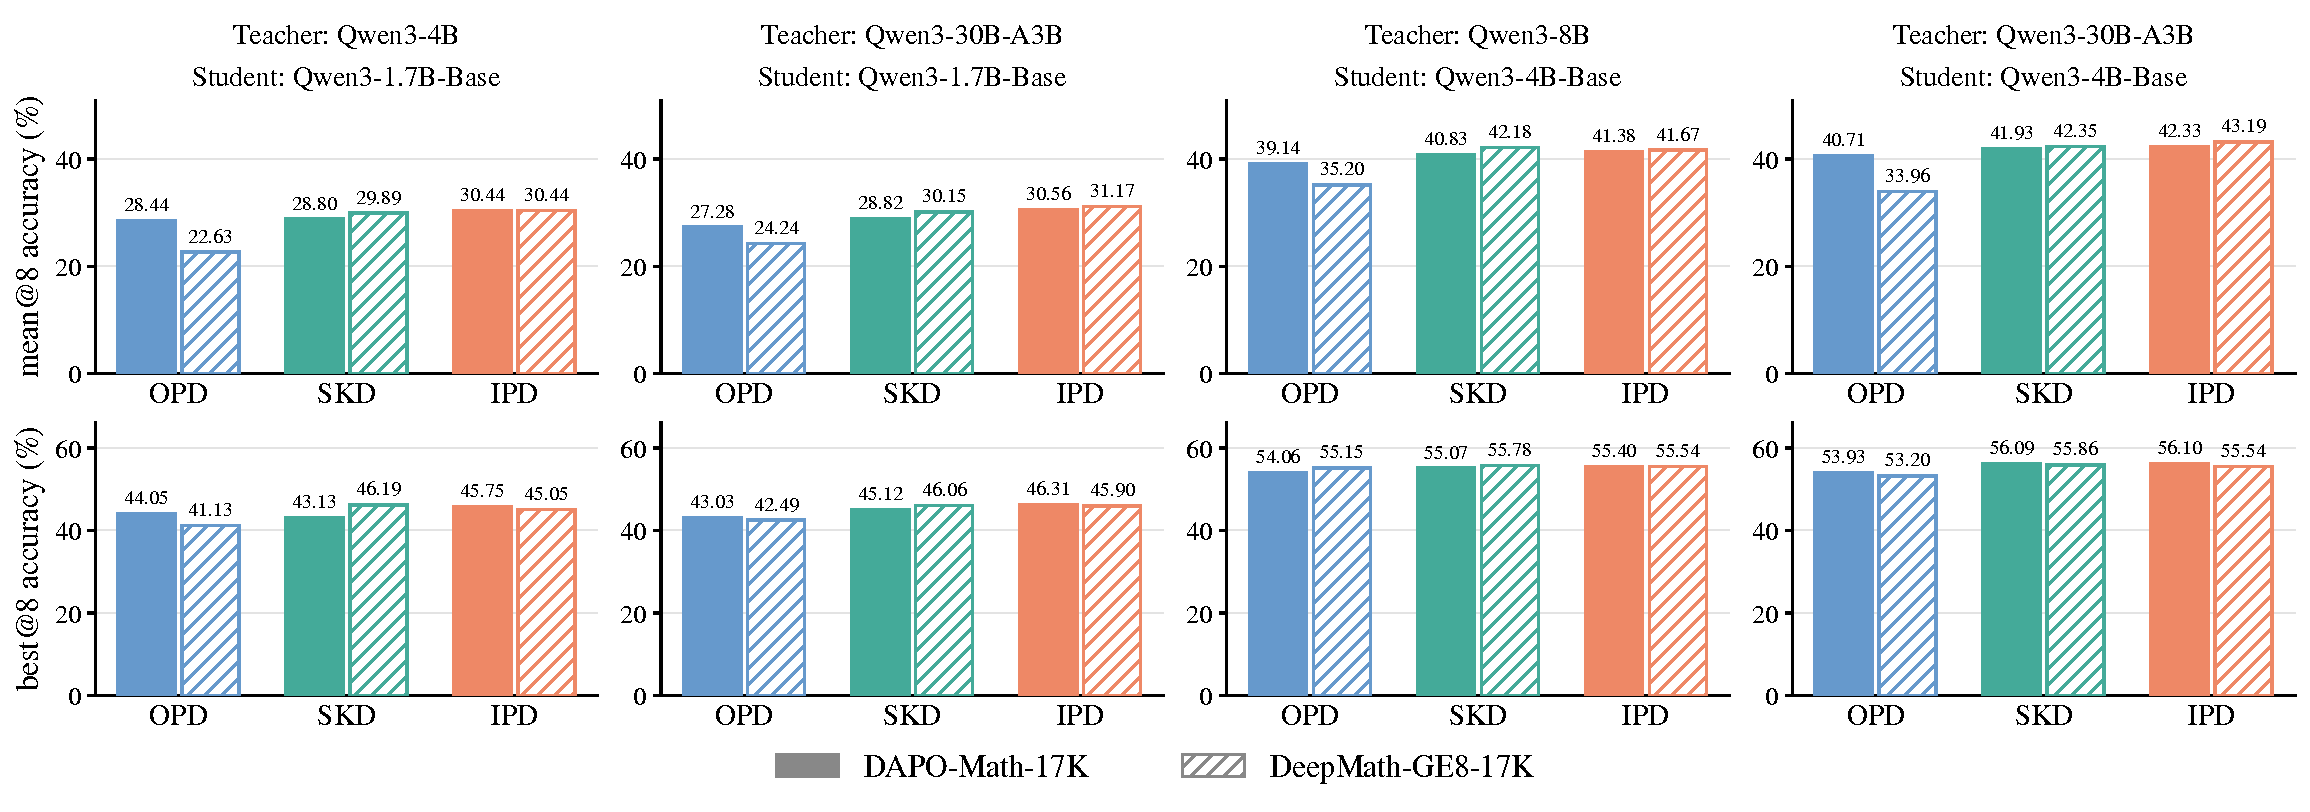
\includegraphics[width=0.99\linewidth]{figures/dataset_comparison_bars.pdf}
  \caption{Comparison of different distillation algorithms on DAPO-MATH-17K and DeepMath-GE8-17K. Intervention-based distillation algorithms including IPD and SKD demonstrate consistent robustness, while OPD apprears to be more sensitive to the change of training data.}
  \label{fig:robustness_on_different_training_data}
\end{figure}

\subsection{Robustness on Different Training Data}
We further explore the robustness of IPD and other distillation algorithms under different training data. In addition to DAPO-MATH-17K, we select examples from DeepMath-103K \citep{he2026deepmath} with difficulty levels greater than or equal to 8 and get 17,085 training examples, denoted as DeepMath-GE8-17K. As shown in Figure~\ref{fig:robustness_on_different_training_data}, we compare different algorithms on these two training datasets. Specifically, we find that algorithms with teacher intervention during rollout, including IPD and SKD, demonstrate a good resistance to the change of training data. 
Meanwhile, OPD shows a non-negligible mean@8 accuracy drop, which indicates that OPD is more sensitive to the training data. On the Qwen3-30B-A3B to Qwen3-4B-Base group, the mean@8 accuracy of OPD even gets a significant drop of $-6.75$. This indicates that without teacher intervention, OPD is more sensitive to the training data, and teacher intervention applied by IPD and SKD can alleviate this sensitivity, which requires less effort on data preparation and makes them more practical paradigms.


\section{Conclusion and Discussion}
In this paper, we propose Interactive-Policy Distillation (IPD), which addresses the teacher unanchoring issue and improve the distillation performance through bidirectional takeover and handback during rollout, together with source-split supervision based on token provenance. This design dynamically corrects trajectories that leave the teacher's acceptance region, and also provides a unified bridge between on-policy and off-policy distillations. Across diverse teacher-student pairs, IPD demonstrates better distillation performance and higher data efficiency, as well as better robustness to training data. We also design a fused inference engine to support our algorithm with efficient dual-model scheduling during the rollout stage.

Currently, like most works in the OPD field, we only consider same-tokenization distillation here. Extending our method to cross-tokenization scenarios is an important problem. Besides, more different rules beyond top-$K$ coverage can be further explored. On the infrastructure side, we only consider synchrnous scheduling for verification and proposal stages. Optimizations like asynchronous scheduling can further improve the throughput of dual-model rollout. We leave these directions for future exploration.

% \newpage
% \subsection*{AI use statement}

% In this work, we have used generative AI tools for training code implementation and optimization, where all the detailed designs were proposed by us. We have not used generative AI tools for fully automated codebase building.
% Additionally, in our manuscript, we have used generative AI tools to refine writing, search related works, and organize experimental results to tables and figures. We have not used generative AI tools to propose research idea of this paper. The research idea is originally proposed by us. 

% \subsection*{Ethics statement}

% There is no significant ethical concern in this work. The datasets and models used in this work are all publicly available.

% \subsection*{Reproducibility statement}

% We have provided a clear description of our proposed method, the necessary experimental settings, and the information of the envirionment where we implement all the experiments. 
% % In addition, we have also included our codebase in the supplementary material. 
% We will also open-source our codebase in the future.


% \subsubsection*{Acknowledgments}
% Use unnumbered third level headings for the acknowledgments. All
% acknowledgments, including those to funding agencies, go at the end of the paper.


\bibliography{iclr2027_conference}
\bibliographystyle{iclr2027_conference}

\newpage
\appendix

\section{Detailed Experimental Settings}
\label{sec:full_exp_details}

\paragraph{Data and models.} We conduct our main experiments on DAPO-Math-17K~\citep{yu2025dapo} with four teacher--student pairs: Qwen3-4B / Qwen3-1.7B-Base, Qwen3-30B-A3B / Qwen3-1.7B-Base, Qwen3-8B / Qwen3-4B-Base, and Qwen3-30B-A3B / Qwen3-4B-Base. Thinking mode is disabled for all teacher models.

\paragraph{Training configuration.} We use the codebase from \citet{li2026rethinking} for OPD, which is under the verl \citep{sheng2025hybridflow} framework. On top of their codebase, we build our fused inference engine and implement SKD and IPD training pipelines. Specifically, as a special case of IPD, SKD also uses our fused inference engine for rollout. Following \citet{li2026rethinking}, unless otherwise specified, we train each model for one epoch (279 steps) with a learning rate of $1\times10^{-6}$. The maximum rollout sequence length is 8192, comprising a maximum prompt length of 1024 and a maximum generation length of 7168. Each prompt produces four training rollouts sampled with temperature 1.0 and top-$p=1.0$. All experiments are conducted on two compute nodes, each equipped with 4 NVIDIA H100 SXM 80GB GPUs. 

\paragraph{Distillation configuration.} All methods use top-$K$ distillation with $K=16$. Each KL term is computed after separately renormalizing the student and teacher distributions over the union support $S_t=S_t^\pi\cup S_t^q$, as defined in Eq.~(\ref{eq:topk_normalization}). IPD and SKD both use $K=16$ for the takeover coverage rule and a proposal length of $\gamma=5$. IPD additionally applies the symmetric top-$K$ coverage rule for handback.

\paragraph{Evaluation.} We evaluate the final checkpoint of every run on MATH-500, Minerva, Olympiad-Bench, AMC23, AIME24, and AIME25. For each problem, we independently sample eight responses with temperature 0.7 and top-$p=0.95$. Same as training, we use a maximum generation length of 7168. We report mean@8 and best@8 accuracy for each benchmark and their benchmark-wise averages. 

\section{Further Discussions}
\subsection{Sampled-Token OPD}
\label{app:sampled_token}

% This section shows that sampled-token OPD is an unbiased estimate of full-vocabulary OPD at every prefix, for both the token-level loss and its gradient, and analyzes the variance incurred by this estimate. 
Since the sampled token follows $x_t\sim\pi_\theta(\cdot\mid c_t)$, taking the expectation of Eq.~(\ref{eq:sampled_token_opd}) over $x_t$ recovers the full-vocabulary reverse KL in Eq.~(\ref{eq:full_vocab_opd}),
\begin{equation}
    \mathbb{E}_{x_t\sim\pi_\theta(\cdot\mid c_t)}\bigl[\widehat{\ell}^{\mathrm{sample}}_t\bigr]
    =\sum_{v\in\mathcal{V}}\pi_\theta(v\mid c_t)\log\frac{\pi_\theta(v\mid c_t)}{q(v\mid c_t)}
    =\ell^{\mathrm{full}}_t .
    \label{eq:sampled_token_unbiased}
\end{equation}
According to \citet{schulman2020approximating}, $\widehat{\ell}^{\mathrm{sample}}_t$ is therefore the $k_1$ estimator of the reverse KL, which is unbiased even though its individual realizations can be negative while $\ell^{\mathrm{full}}_t\geq 0$ is guaranteed.
Given the identity $\nabla_\theta\pi_\theta(v\mid c_t)=\pi_\theta(v\mid c_t)\nabla_\theta\log\pi_\theta(v\mid c_t)$,
the product rule applied to Eq.~(\ref{eq:full_vocab_opd}) gives
\begin{equation}
\begin{aligned}
    \nabla_\theta\ell^{\mathrm{full}}_t
    &=\sum_{v\in\mathcal{V}}\nabla_\theta\pi_\theta(v\mid c_t)\,
      \log\frac{\pi_\theta(v\mid c_t)}{q(v\mid c_t)}
      +\sum_{v\in\mathcal{V}}\pi_\theta(v\mid c_t)\nabla_\theta\log\frac{\pi_\theta(v\mid c_t)}{q(v\mid c_t)}\\
    &=\sum_{v\in\mathcal{V}}\nabla_\theta\pi_\theta(v\mid c_t)\,
      \log\frac{\pi_\theta(v\mid c_t)}{q(v\mid c_t)}
      +\sum_{v\in\mathcal{V}}\nabla_\theta\pi_\theta(v\mid c_t)\\
    &=\sum_{v\in\mathcal{V}}\nabla_\theta\pi_\theta(v\mid c_t)\,
      \log\frac{\pi_\theta(v\mid c_t)}{q(v\mid c_t)}
      +\nabla_\theta\sum_{v\in\mathcal{V}}\pi_\theta(v\mid c_t)\\
    &=\sum_{v\in\mathcal{V}}\pi_\theta(v\mid c_t)\log\frac{\pi_\theta(v\mid c_t)}{q(v\mid c_t)}\nabla_\theta\log\pi_\theta(v\mid c_t)
      +\nabla_\theta 1\\
    &=\mathbb{E}_{x_t\sim\pi_\theta(\cdot\mid c_t)}\Bigl[\widehat{\ell}^{\mathrm{sample}}_t\,
      \nabla_\theta\log\pi_\theta(x_t\mid c_t)\Bigr].
\end{aligned}
\label{eq:full_vocab_grad}
\end{equation}
We denote the gradient estimator as
\begin{equation}
    \widehat{g}_t=\widehat{\ell}^{\mathrm{sample}}_t\,
    \nabla_\theta\log\pi_\theta(x_t\mid c_t). 
    \label{eq:sampled_token_grad}
\end{equation}
Under the context of gradient ascent in reinforcement learning, $-\widehat{g}_t$ is the policy gradient obtained when OPD is implemented as maximizing
\begin{equation}
\begin{aligned}
  \mathcal{J}_t = \mathbb{E}_{x_t\sim\pi_\theta(\cdot\mid c_t)}\Bigl[\text{sg}\big[-\widehat{\ell}^{\mathrm{sample}}_t\big]\Bigr],
\end{aligned} 
\end{equation}
where the per-token reward is the stop-gradient operated $-\widehat{\ell}^{\mathrm{sample}}_t = \log q(x_t\mid c_t)-\log\pi_\theta(x_t\mid c_t)$ \citep{lu2025onpolicydistillation, oh2026klforkl}. 
% The stop-gradient is indispensable, because differentiating $\widehat{\ell}^{\mathrm{sample}}_t$ with $x_t$ held fixed would instead yield $\nabla_\theta\log\pi_\theta(x_t\mid c_t)$, whose expectation under $\pi_\theta(\cdot\mid c_t)$ is zero. Moreover, both sampled-token and full-vocabulary OPD treat the sampled prefixes as constants and do not backpropagate through the student's sampling distribution \citep{gkd}, so the unbiasedness established above holds prefix by prefix. Retaining the dependence of the prefixes on $\theta$, as the exact gradient of Eq.~(\ref{eq:on_policy_kd}) would require, couples each token with all subsequent rewards and further increases the variance \citep{fu2026revisiting}.

Given a prefix $c_t$, variances of the sampled-token loss and gradient are
\begin{align}
    \operatorname{Var}\bigl[\widehat{\ell}^{\mathrm{sample}}_t\mid c_t\bigr]
    &=\sum_{v\in\mathcal{V}}\pi_\theta(v\mid c_t)
      \left(\log\frac{\pi_\theta(v\mid c_t)}{q(v\mid c_t)}\right)^2
      -\bigl(\ell^{\mathrm{full}}_t\bigr)^2
    \nonumber\\
    &=\sum_{v\in\mathcal{V}}\pi_\theta(v\mid c_t)
      \left(\log\frac{\pi_\theta(v\mid c_t)}{q(v\mid c_t)}
      -\ell^{\mathrm{full}}_t\right)^2,
    \label{eq:sampled_token_variance}\\
    \operatorname{Var}\bigl[\widehat{g}_t\mid c_t\bigr]
    &=\mathbb{E}\bigl[\|\widehat{g}_t-\nabla_\theta\ell^{\mathrm{full}}_t\|^2\mid c_t\bigr]\nonumber\\
    &=\mathbb{E}\bigl[(\widehat{\ell}^{\mathrm{sample}}_t)^2
      \|\nabla_\theta\log\pi_\theta(x_t\mid c_t)\|^2\mid c_t\bigr]
      -\|\nabla_\theta\ell^{\mathrm{full}}_t\|^2
    \nonumber\\
    &=\sum_{v\in\mathcal{V}}\pi_\theta(v\mid c_t)
      \left\|\log\frac{\pi_\theta(v\mid c_t)}{q(v\mid c_t)}
      \nabla_\theta\log\pi_\theta(v\mid c_t)
      -\nabla_\theta\ell^{\mathrm{full}}_t\right\|^2.
    \label{eq:sampled_token_grad_variance}
\end{align}

Eq.~(\ref{eq:sampled_token_variance}) and Eq.~(\ref{eq:sampled_token_grad_variance}) reveal a common source of variance in sampled-token OPD.
When the teacher and student disagree strongly, the student may assign much higher probability to tokens with $q(v\mid c_t)\ll\pi_\theta(v\mid c_t)$, yielding much larger log-ratios than on tokens where the models agree \citep{fu2026revisiting}. Sampling among these tokens makes the loss and gradient fluctuate, leading to noisy and potentially unstable updates \citep{oh2026klforkl}.
% Eq.~(\ref{eq:sampled_token_variance}) shows that the sampled-token loss variance is large when tokens with appreciable student probability have log-ratios far from $\ell^{\mathrm{full}}_t$. In particular, when there is a large difference between the teacher and student distributions, at some index $v$ the student will have a much higher probability than the teacher, \emph{i.e.}, $q(v\mid c_t)\ll\pi_\theta(v\mid c_t)$, and it can produce a very large positive log-ratios for those tokens sampled by the student. 
% Eq.~(\ref{eq:sampled_token_grad_variance}) gives the corresponding condition for gradient variance: the log-ratio-weighted score must deviate substantially from $\nabla_\theta\ell^{\mathrm{full}}_t$, with sufficient student probability. Thus a small teacher probability alone does not imply high variance; its effect depends on the student probability, the score vector $\nabla_\theta\log\pi_\theta(v\mid c_t)$, and the deviation from the mean. 
% These expressions explain how teacher-student gap can yield noisy sampled-token updates \citep{fu2026revisiting, oh2026klforkl}.

\subsection{Distillation Support} 
According to the GitHub issue discussion from the official repository of \citet{li2026rethinking}, different choices of support (including $S_t^\pi$, $S_t^q$, $S_t^\pi\cup S_t^q$, and $S_t^\pi\cap S_t^q$) do not bring significant differences for same-size distillation. From our observation, for different-size distillation, using the union of the two top-$K$ sets $S_t^\pi\cup S_t^q$ as the support for top-$K$ OPD is slightly better than using others. Unless specified, we use the union of the two top-$K$ sets by default in this paper.

\subsection{Loss Aggregation}
Following GKD~\citep{gkd} and SKD~\citep{skd}, Eq.~(\ref{eq:ipd_objective}) uses a sequence-mean-token-mean aggregation, which assigns equal weight to each response and prevents longer reasoning traces from dominating the minibatch objective. Another aggregation commonly used in OPD implementations is the global token mean, which assigns equal weight to every valid token and consequently weights each rollout in proportion to its length. This aggregation choice is orthogonal to the rollout policy, the token source, and the direction of the source-split KL. From our practice, global token-mean aggregation and sequence-mean-token-mean aggregation produce comparable performances, while the latter yields slightly more stable optimization. We therefore use sequence-mean-token-mean aggregation by default in this paper. 

\subsection{Student Models}
In this paper, we use Qwen3 Base models as student for all the experiments. Non-base Qwen3 models are trained to switch between thinking mode and non-thinking mode within single model, and this switch is contorlled by special $\langle\text{think}\rangle$ and $\langle/\text{think}\rangle$ tokens. Specifically, when disabling thinking mode, the tokenizer will append an empty $\langle\text{think}\rangle\langle/\text{think}\rangle$ block to the prompt before decoding. If using non-base Qwen3 models with thinking mode disabledas student, it can be difficult to distinguish whether the student performance gain is from successfully aligning with the teacher, or it just somehow manages to bypass the template-controlled thinking mode switch and silently activates its thinking capability obtained from previous training. Therefore, if using non-base Qwen3 models with thinking mode disabled as teacher, we think using Qwen3 Base models as student is a cleaner setting for distillation experiments. Another clean setting is to use non-base Qwen3 models with thinking mode enabled as both teacher and student, but this setting would require a much longer response length and consume more computational resources. We leave this setting for future exploration.

\section{Additional Experimental Results}

\subsection{Additional Main Results}
In addition to the main results in Table~\ref{tab:main_results}, we also report the mean@8 accuracy and top-$K$ overlap ratio curves during training, as shown in Figure~\ref{fig:qwen3_all_group_curves}.

\begin{figure}[!h]
  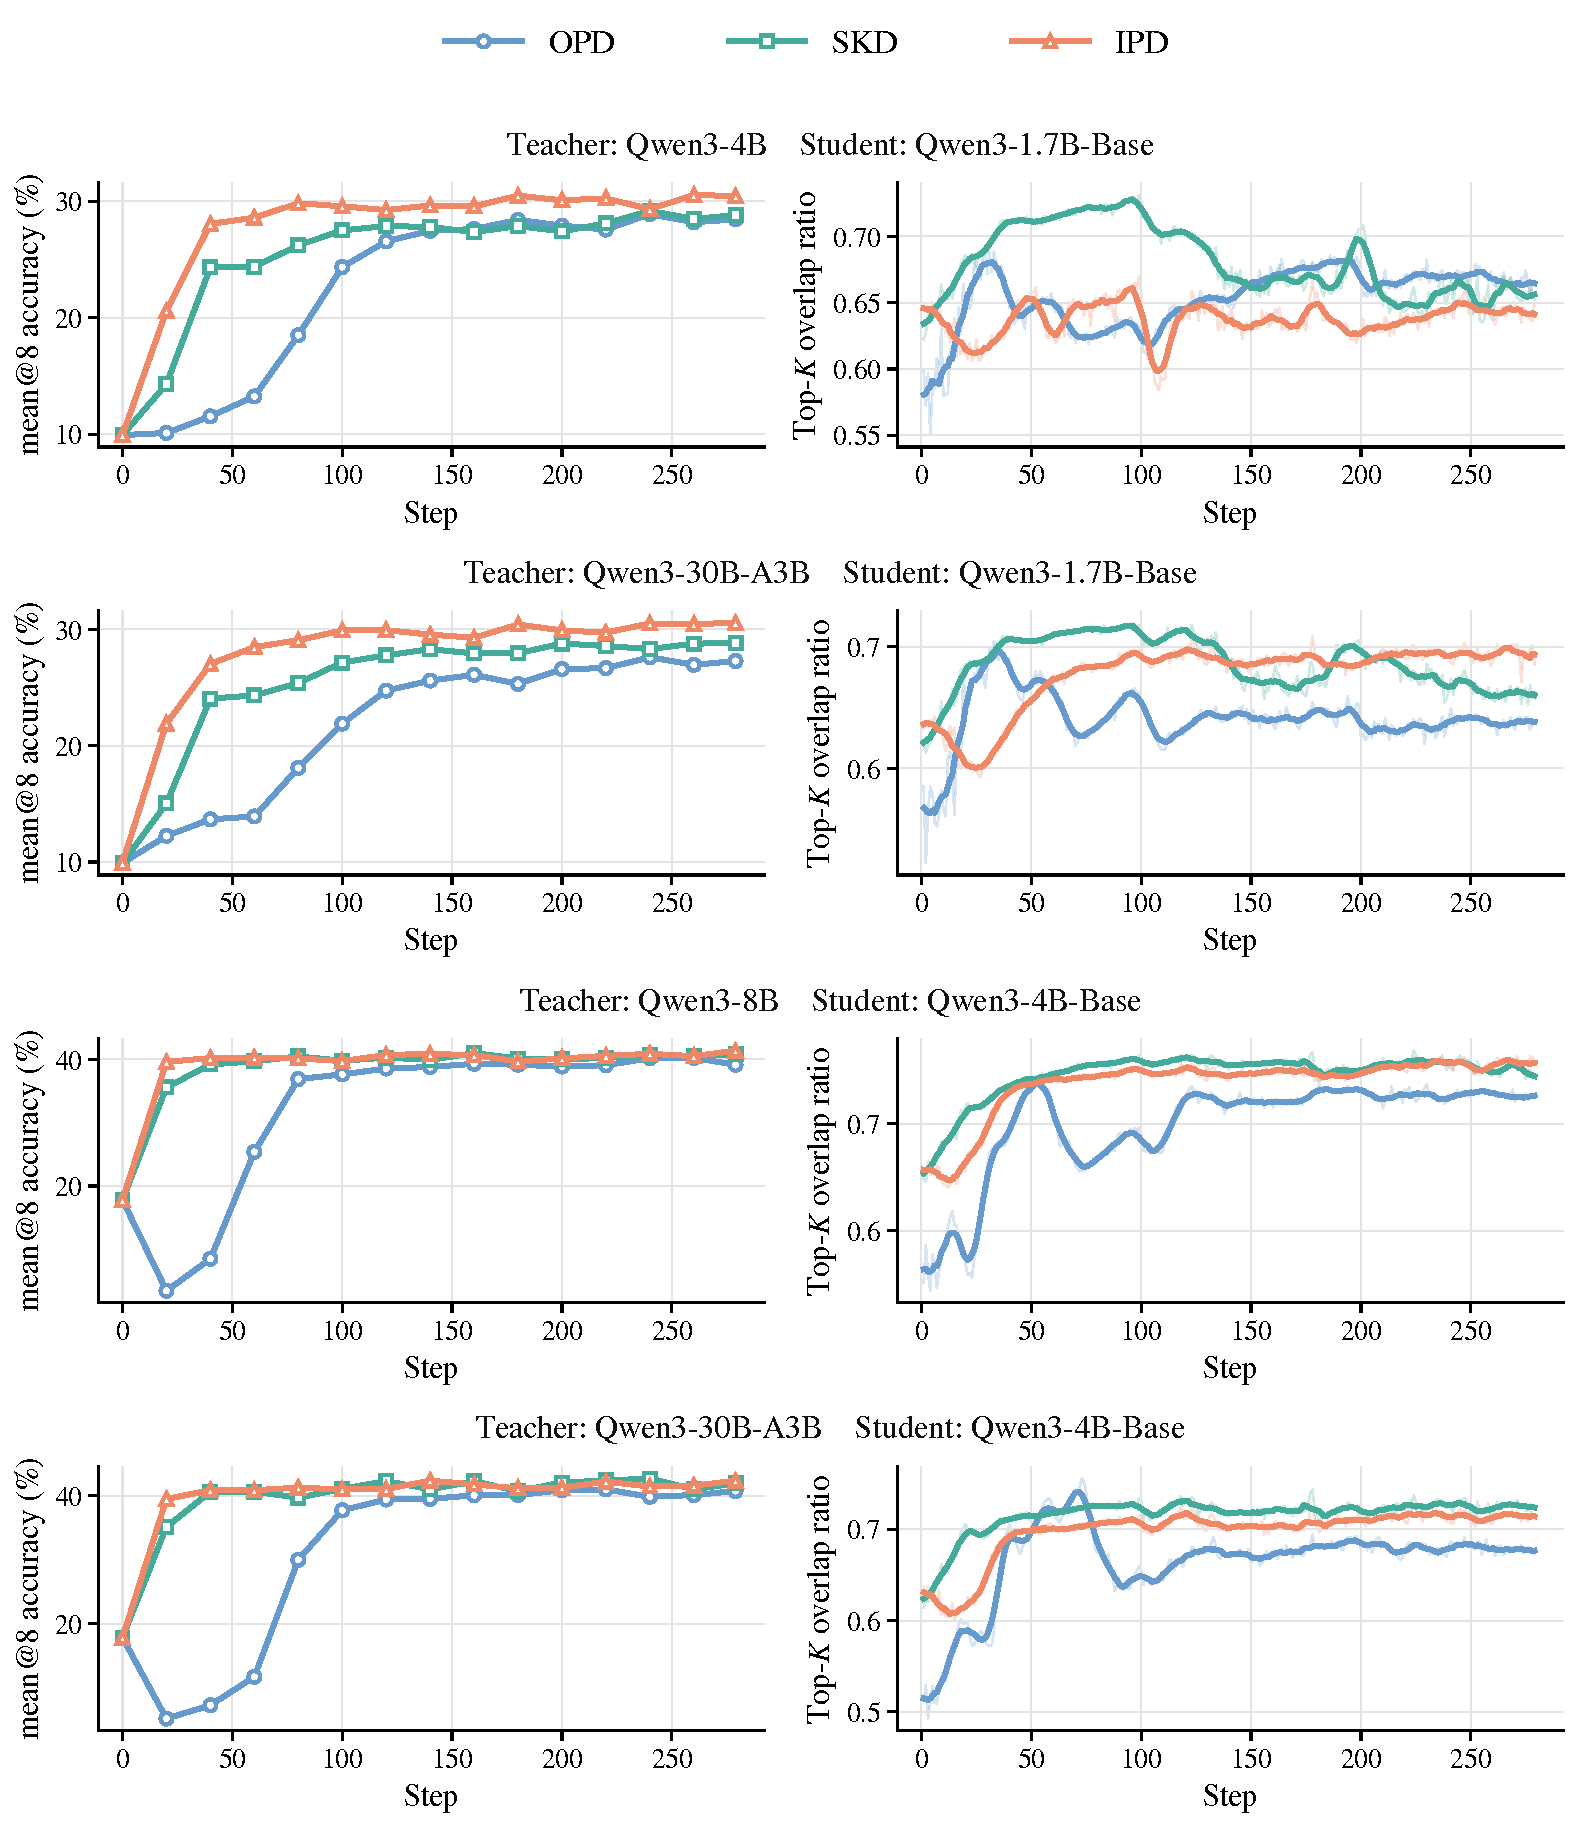
\includegraphics[width=0.99\linewidth]{figures/curves_four_groups.pdf}
  \caption{The mean@8 accuracy and top-$K$ overlap ratio curve for four groups of models.}
  \label{fig:qwen3_all_group_curves}
\end{figure}
\FloatBarrier

\subsection{Additional Ablation Results}
\label{sec:ablation_details}

\paragraph{KL direction.} Table~\ref{tab:ablation_loss} shows that the default source-split KL obtains the highest benchmark-averaged mean@8 accuracy ($30.44$), while pure reverse KL has a slightly higher best@8 ($45.87$) than default ($45.75$). 

\begin{table}[!ht]
\centering
\small
\caption{Benchmark-wise mean@8 and best@8 accuracy for the KL-direction ablation.}
\label{tab:ablation_loss}
\resizebox{\textwidth}{!}{%
\begin{tabular}{l cc cc cc cc cc cc cc}
\toprule
& \multicolumn{2}{c}{MATH-500} & \multicolumn{2}{c}{Minerva} & \multicolumn{2}{c}{Olympiad} & \multicolumn{2}{c}{AMC23} & \multicolumn{2}{c}{AIME24} & \multicolumn{2}{c}{AIME25} & \multicolumn{2}{c}{\textbf{Avg.}} \\
\cmidrule(lr){2-3} \cmidrule(lr){4-5} \cmidrule(lr){6-7} \cmidrule(lr){8-9} \cmidrule(lr){10-11} \cmidrule(lr){12-13} \cmidrule(lr){14-15}
Loss Variant & mean@8 & best@8 & mean@8 & best@8 & mean@8 & best@8 & mean@8 & best@8 & mean@8 & best@8 & mean@8 & best@8 & mean@8 & best@8 \\
\midrule
Pure Reverse KL & 68.23 & 84.05 & 29.18 & 46.21 & \textbf{32.13} & 49.70 & 35.39 & 56.46 & \textbf{10.42} & \textbf{27.24} & 4.17 & 11.56 & 29.92 & \textbf{45.87} \\
Pure Forward KL & 66.80 & 83.64 & 28.77 & 45.15 & 30.46 & 49.69 & 34.19 & \textbf{58.58} & 6.67 & 18.41 & 4.17 & 11.60 & 28.51 & 44.51 \\
Inverse-IPD-Split KL & 67.35 & \textbf{84.84} & 27.16 & 44.06 & 31.37 & \textbf{50.31} & 33.58 & 56.63 & 9.17 & 22.66 & \textbf{6.67} & \textbf{15.09} & 29.22 & 45.60 \\
IPD-Split KL (default) & \textbf{69.28} & 84.59 & \textbf{29.60} & \textbf{46.26} & 31.80 & 49.63 & \textbf{36.14} & 57.25 & 9.17 & 21.69 & \textbf{6.67} & 15.06 & \textbf{30.44} & 45.75 \\
\bottomrule
\end{tabular}}
\end{table}

\paragraph{Coverage width.} Table~\ref{tab:ablation_k_values} shows that $K=4$ yields the highest average mean@8 and best@8, but only slightly exceeds the default $K=16$ by $+0.02$ and $+0.05$, respectively.

\begin{table}[!ht]
\centering
\small
\caption{Benchmark-wise mean@8 and best@8 accuracy for the top-$K$ coverage ablation.}
\label{tab:ablation_k_values}
\resizebox{\textwidth}{!}{%
\begin{tabular}{l cc cc cc cc cc cc cc}
\toprule
& \multicolumn{2}{c}{MATH-500} & \multicolumn{2}{c}{Minerva} & \multicolumn{2}{c}{Olympiad} & \multicolumn{2}{c}{AMC23} & \multicolumn{2}{c}{AIME24} & \multicolumn{2}{c}{AIME25} & \multicolumn{2}{c}{\textbf{Avg.}} \\
\cmidrule(lr){2-3} \cmidrule(lr){4-5} \cmidrule(lr){6-7} \cmidrule(lr){8-9} \cmidrule(lr){10-11} \cmidrule(lr){12-13} \cmidrule(lr){14-15}
Coverage width & mean@8 & best@8 & mean@8 & best@8 & mean@8 & best@8 & mean@8 & best@8 & mean@8 & best@8 & mean@8 & best@8 & mean@8 & best@8 \\
\midrule
$K=4$ & 68.30 & \textbf{85.36} & 28.49 & 43.59 & 31.97 & 49.76 & 35.24 & 53.75 & \textbf{10.00} & \textbf{24.21} & \textbf{8.75} & \textbf{18.17} & \textbf{30.46} & \textbf{45.80} \\
$K=8$ & 69.20 & 84.94 & 28.95 & 45.00 & 32.45 & \textbf{50.97} & 33.43 & 54.60 & 8.75 & 17.68 & 6.25 & 14.10 & 29.84 & 44.55 \\
\textbf{$K=16$}~~\small\textbf{(default)} & \textbf{69.28} & 84.59 & \textbf{29.60} & \textbf{46.26} & 31.80 & 49.63 & \textbf{36.14} & \textbf{57.25} & 9.17 & 21.69 & 6.67 & 15.06 & 30.44 & 45.75 \\
$K=32$ & 68.03 & 83.81 & 28.77 & 44.66 & \textbf{32.50} & 50.50 & 34.64 & 53.96 & 8.75 & 17.58 & 5.42 & 14.30 & 29.68 & 44.13 \\
\bottomrule
\end{tabular}}
\end{table}
\FloatBarrier


\section{Same-origin Distillation}
In addition to different models from the Qwen3 family, we also conduct a same-origin distillation experiment with DeepSeek-R1-Distill-Qwen-1.5B as the student and JustRL-DeepSeek-1.5B as the teacher. Specifically, JustRL-DeepSeek-1.5B is the further post-trained version of DeepSeek-R1-Distill-Qwen-1.5B via simple GRPO recipe \citep{he2025justrl}. The results are shown in Table~\ref{tab:same_origin} and Figure~\ref{fig:same_origin}. We find that intervention methods including IPD and SKD do not bring as statistically significant improvement over OPD compared with our main experiments with different-size Qwen3 models. From Figure~\ref{fig:same_origin}, we can observe that the mean@8 accuracy and top-$K$ overlap ratio curves of three methods are very close to each other's, which is expected as the student and teacher are same-origin models. The same-origin experiment indicates that OPD can already achieve a good distillation performance when the reasoning gap between the student and teacher are not significant, which is consistent with the discussion from \citet{li2026rethinking}, and the main advantage of IPD remains in large-gap distillation scenarios.

\begin{table}[!h]
\setlength{\aboverulesep}{0pt}
\setlength{\belowrulesep}{0pt}
\setlength{\extrarowheight}{2pt}
\centering
\small
\caption{Same-origin distillation experiment with DeepSeek-R1-Distill-Qwen-1.5B as the student and JustRL-DeepSeek-1.5B as the teacher on DAPO-Math-17K-Processed. Intervention methods including IPD and SKD do not bring as statistically significant improvement over OPD compared with our main experiments with different-size Qwen3 models.}
\label{tab:same_origin}
\resizebox{\textwidth}{!}{%
\begin{tabular}{ll cc cc cc cc cc cc cc}
\toprule
\multicolumn{1}{c}{\multirow{2}{*}{\makecell{Teacher/\\Student}}} & \multicolumn{1}{c}{\multirow{2}{*}{Method}} & \multicolumn{2}{c}{MATH-500} & \multicolumn{2}{c}{Minerva} & \multicolumn{2}{c}{Olympiad} & \multicolumn{2}{c}{AMC23} & \multicolumn{2}{c}{AIME24} & \multicolumn{2}{c}{AIME25} & \multicolumn{2}{c}{\textbf{Avg.}} \\
\cmidrule(lr){3-4} \cmidrule(lr){5-6} \cmidrule(lr){7-8} \cmidrule(lr){9-10} \cmidrule(lr){11-12} \cmidrule(lr){13-14} \cmidrule(lr){15-16}
& & mean@8 & best@8 & mean@8 & best@8 & mean@8 & best@8 & mean@8 & best@8 & mean@8 & best@8 & mean@8 & best@8 & mean@8 & best@8 \\
\midrule
\multirow{3}{*}{\makecell[l]{JustRL-DeepSeek-1.5B/\\DeepSeek-R1-Distill-\\Qwen-1.5B}} & OPD & 85.15 & 92.79 & \textbf{38.01} & 49.41 & 47.29 & 60.63 & \textbf{64.16} & \textbf{82.92} & 27.50 & \textbf{52.85} & 20.83 & 30.59 & 47.16 & \textbf{61.53} \\
& SKD & 85.55 & \textbf{93.36} & 37.13 & 47.80 & \textbf{48.74} & \textbf{61.70} & 63.55 & 79.67 & 27.92 & 50.43 & \textbf{23.33} & \textbf{32.58} & 47.70 & 60.92 \\
& \ipdcell{\textbf{IPD (ours)}} & \ipdcell{\textbf{85.75}} & \ipdcell{93.29} & \ipdcell{37.78} & \ipdcell{\textbf{49.99}} & \ipdcell{48.11} & \ipdcell{61.36} & \ipdcell{62.80} & \ipdcell{79.53} & \ipdcell{\textbf{30.42}} & \ipdcell{47.13} & \ipdcell{22.92} & \ipdcell{29.80} & \ipdcell{\textbf{47.96}} & \ipdcell{60.18} \\
\bottomrule
\end{tabular}}
\end{table}

\begin{figure}[!h]
  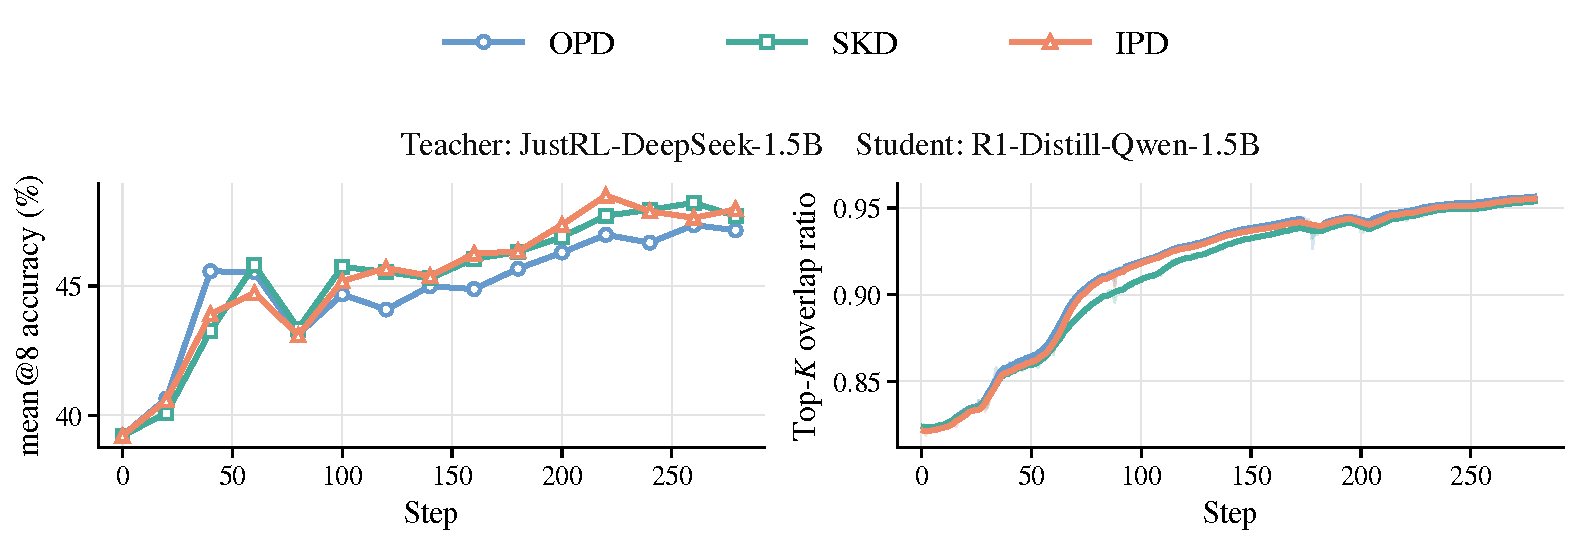
\includegraphics[width=0.99\linewidth]{figures/curves_same_origin.pdf}
  \caption{The mean@8 accuracy and top-$K$ overlap ratio curve for same-origin distillation experiment with DeepSeek-R1-Distill-Qwen-1.5B as the student and JustRL-1.5B as the teacher. }
  \label{fig:same_origin}
\end{figure}

\section{Distillation on Limited Trainig Examples}
We also run distillation trainings on limited training examples to evaluate the impact of data scarcity on the distillation process. Specifically, we randomly select 1,024 training examples from DAPO-MATH-17K and conduct distillation experiments using Qwen3-4B as teacher and Qwen3-1.7B-Base as student. The student model is trained for 15 epochs (with 240 steps in total), and the other training configurations remains the same as the main experiments. 
The results are shown in Figure~\ref{fig:limited_data}. We find that IPD can still outperform OPD and SKD and shows a higher convergence under limited training data. Another interesting observation is that, even if the training examples only count for about 1/17 of the original training data, all the three methods can matches the performance of the student model trained on the full training dataset. The limited training data experiment indicates that although with limited unique training prompts, as long as they can be replayed to generate diverse rollouts, the distillation can still be effective. 

\begin{figure}[!h]
  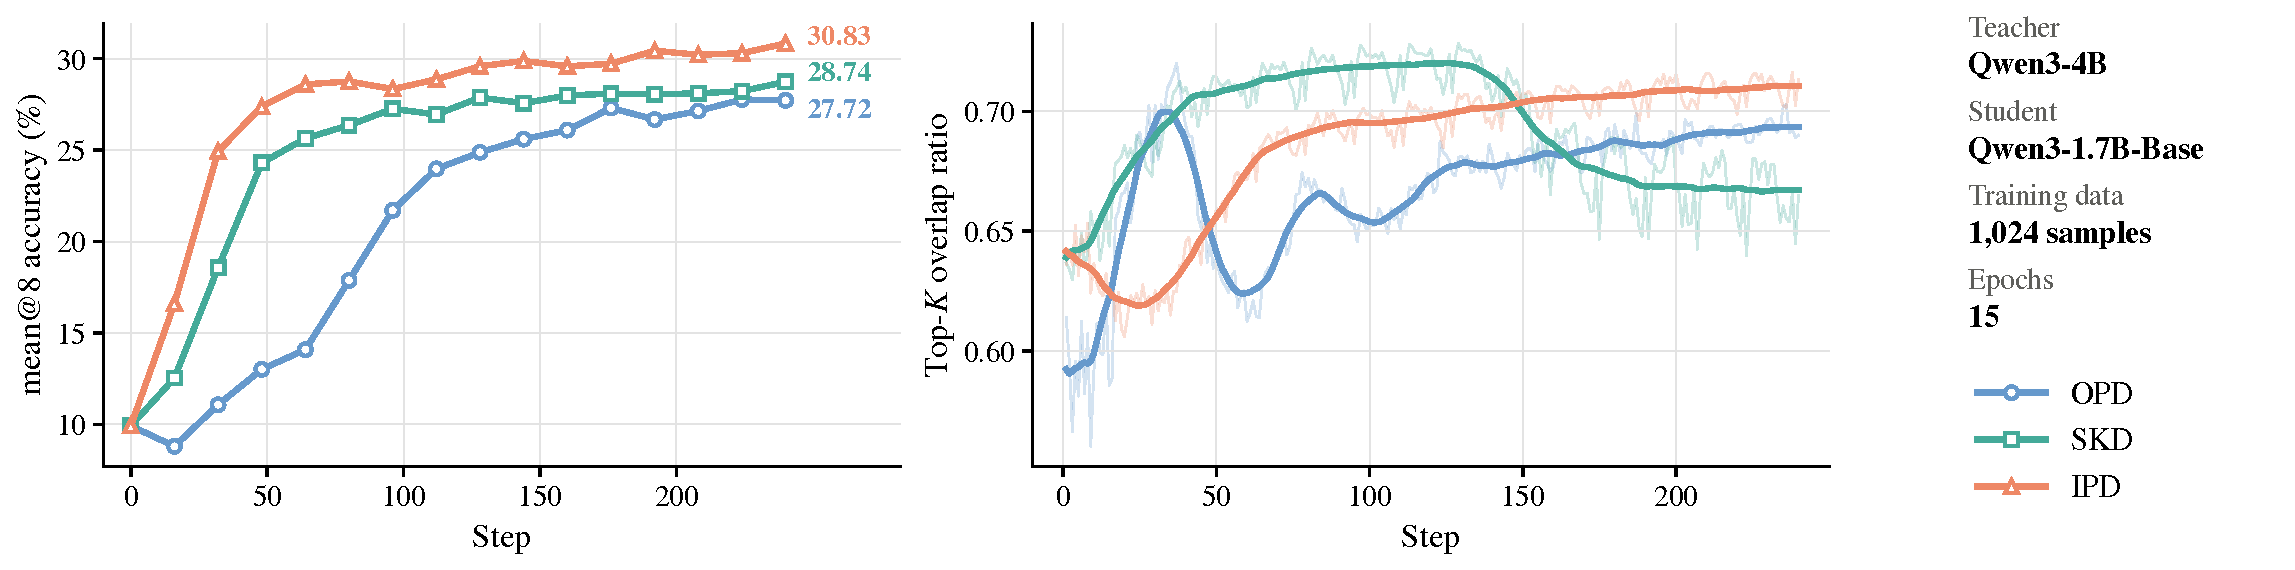
\includegraphics[width=0.99\linewidth]{figures/curves_limited_data.pdf}
  \caption{The mean@8 accuracy and top-$K$ overlap ratio curve for distillation on 1,024 randomly selected DAPO-MATH-17K training examples. As long as the limited unique training prompts can be replayed to generate diverse rollouts, the distillation can still be effective.}
  \label{fig:limited_data}
\end{figure}

\end{document}
